\conditionalgeometry
% each figure gets its own page so that we can extract it into a separate eps file.
\makeatletter
\@fpsep\textheight
\makeatother
% no page numbers on figure files
\section{} % Figures
% \newgeometry{left=1cm,right=1cm} can be used if you have big figures that come all the way out to the edge of the page. But it's better to stick with nice 1" margins and then use a special landscape page for any wide figures.
\singlespacing % Very important for figure captions and Texshade
\setcounter{figure}{0}
\renewcommand{\figurename}{Fig.}
\renewcommand{\thefigure}{\arabic{figure}}
\begin{figure}[!h]
\centering
%\figuretitle{Figure~\ref{fig:S173I_genetics_and_biochemistry}}
\begin{conditionalpanel}
    \begin{tikzcanvas}{}
        %
        \node(pedigree)[inner sep=0pt] at (current page.north) {\includegraphics[width=\linewidth,height=2.75in,keepaspectratio]{../results/pedigree_S173I/output/pedigree_S173I_standalone.pdf}};
        %
        \node(captionA)[inner sep=0pt,above left] at (pedigree.north west) {\normalsize\textbf{\figurepanela}};
        %
        %
        %
        \node(S173I_plot)[inner sep=0pt,below=3.25cm of pedigree.south west,anchor=west]{\input{../results/assembly_kinetics/output/kinetics_CPVT_mutation_S173I_85mM_K.pgf}};
        %
        \node(captionB)[inner sep=0pt,above left] at (S173I_plot.north west) {\normalsize\textbf{\figurepanelb}};
        %
        %
        %
        \node(K180R_plot)[inner sep=0pt,right=0.75cm of S173I_plot]{\input{../results/assembly_kinetics/output/kinetics_CPVT_mutation_K180R_85mM_K.pgf}};
        %
        \node(captionC)[inner sep=0pt,above left] at (K180R_plot.north west) {\normalsize\textbf{\figurepanelc}};
        %
        %
        %
        \node(K180RMg_plot)[inner sep=0pt,below=3.25cm of S173I_plot.south west,anchor=west]{\input{../results/assembly_kinetics/output/kinetics_CPVT_mutations_K180R_Mg.pgf}};
        %
        \node(captionD)[inner sep=0pt,above left] at (K180RMg_plot.north west) {\normalsize\textbf{\figurepaneld}};
    \end{tikzcanvas}
\end{conditionalpanel}
\begin{conditionalcaption}
\caption[Dominant cardiac calsequestrin disease mutations]{\textbf{\headingsubsectionone}. \figurepanelcaptiona Pedigree of a large extended family with the S173I mutation and a CPVT-like phenotype. CABG = coronary artery bypass graft; CAD = coronary artery disease; CHD = congenital heart disease; ETT = exercise treadmill test; MI = myocardial infarction; SCD = sudden cardiac death; SIDS = sudden infant death syndrome. \figurepanelcaptionb Multimerization kinetics of the S173I mutant observed using a turbidity assay after addition of \SI{1}{\milli\Molar} \ch{CaCl2} to purified protein (pH 7.4, \SI{20}{\milli\Molar} NaCl, \SI{85}{\milli\Molar} KCl). \figurepanelcaptionc Multimerization kinetics of the K180R mutant observed using a turbidity assay (same conditions as in \textbf{b}). \figurepanelcaptiond Multimerization kinetics of the K180R mutant observed using a turbidity assay (same conditions as in \figurepanelcaptionb but with \SI{2}{\milli\Molar} \ch{MgCl2} added prior to calcium). All graphed values are mean of 3 technical replicates ± SD.}
\label{fig:S173I_genetics_and_biochemistry}
\end{conditionalcaption}
\end{figure}
\newcommand{\colorDomainI}{pymolpurple}
\newcommand{\colorDomainII}{pymolgreencyan}
\newcommand{\colorDomainIII}{pymolslate}
\begin{figure}[!h]
\centering
%\figuretitle{Figure~\ref{fig:filament_overview}}
\begin{conditionalpanel}
    \begin{tikzcanvas}{}
        \node(filament)[inner sep=0pt,below right]{\includegraphics[width=\linewidth,height=1.25in,keepaspectratio]{../results/filament_overview/output/overview_surface_cropped.png}};
        %
        \node(captionA)[inner sep=0pt,above left] at (filament.north west) {\normalsize\textbf{\figurepanela}};
        %
        \path (filament.south)++(-1,3.15) coordinate (filament_dimer_NW);
        \path (filament.south)++(1,1) coordinate (filament_dimer_SE);
        %
        \path (filament.south)++(-1,3.15) coordinate (filament_tetramer_NW);
        \path (filament.south)++(2.7,0.5) coordinate (filament_tetramer_SE);
        %
        \node(dimerrectfilament) [fit={(filament_dimer_NW) (filament_dimer_SE)}, dashedrectanglefit] {};
        %
        \node(dimer_dimer_rect_filament) [fit={(filament_tetramer_NW) (filament_tetramer_SE)}, dashedrectanglefit] {};
        %
        %
        %
        %
        \node(dimer)[inner sep=0pt,right=1.5cm of filament]{\includegraphics[width=\linewidth,height=1.25in,keepaspectratio]{../results/filament_overview/output/overview_dimer_cropped.png}};
        %
        \node(dimerrect) [fit=(dimer), dashedrectanglefit] {};
        \node(dimer_caption)[above, inner sep=7pt] at (dimer.north) {Dimer};
        %        
        \node(dimer_chainAlabel)[above, inner sep=0pt] at ([shift={(-0.125cm,-0.6cm)}]dimer.south west) {Chain A};
%        \draw[] ([shift={(0cm,0.125cm)}]dimer_chainAlabel.north) -- ([shift={(0.25cm,0.125cm)}]dimer.south west);
        %
        \node(dimer_chainBlabel)[above, inner sep=0pt] at ([shift={(0.125cm,-0.6cm)}]dimer.south east) {Chain B};
%        \draw[] ([shift={(0cm,0.125cm)}]dimer_chainBlabel.north) -- ([shift={(-0.25cm,0.125cm)}]dimer.south east);
        % \path (dimer.south west)++(0,-0.5) coordinate (chainA);
        % \path (dimer.south east)++(0,-0.5) coordinate (chainB);
        % %
        % \node(chainAlabel) [above, inner sep=2pt, align=center] at (chainA) {Chain A};
        % \node(chainBlabel) [above, inner sep=2pt, align=center] at (chainB) {Chain B};
        % %
        %
        %
        \node(dimer_dimer)[inner sep=0pt,below=1.5cm of dimer.south,anchor=north]{\includegraphics[width=\linewidth,height=1.5in,keepaspectratio]{../results/filament_overview/output/overview_tetramer_cropped.png}};
        %
        \node(dimer_dimer_rect) [fit=(dimer_dimer), dashedrectanglefit] {};
        %
        % \path (dimer_dimer.north east)++(0,0) coordinate (dimer_dimer_chainA);
        % \path (dimer_dimer.south east)++(0.75,1) coordinate (dimer_dimer_chainB);
        % \path (dimer_dimer.north)++(1.5,-0.5) coordinate (dimer_dimer_chainAprime);
        % \path (dimer_dimer.south east)++(0.75,1) coordinate (dimer_dimer_chainBprime);
        %
        % \node(dimer_dimer_chainAlabel)[above, inner sep=0pt] at ([shift={(-0.25cm,0.75cm)}]dimer_dimer.north west) {Chain A};
        % \draw[] ([shift={(0cm,-0.25cm)}]dimer_dimer_chainAlabel.south) -- ([shift={(0.25cm,-0.125cm)}]dimer_dimer.north west);
        % %
        % \node(dimer_dimer_chainBlabel)[above, inner sep=0pt] at ([shift={(-0.25cm,0.5cm)}]dimer_dimer.north) {Chain B};
        % \draw[] ([shift={(0cm,-0.25cm)}]dimer_dimer_chainBlabel.south) -- ([shift={(-0.25cm,-0.125cm)}]dimer_dimer.north);
        %
        \node(dimer_dimer_chainAprimelabel)[above, inner sep=2pt] at ([shift={(1.5cm,-0.75cm)}]dimer_dimer.north) {Chain A'};
        %\draw[] ([shift={(0cm,0cm)}]dimer_dimer_chainAprimelabel.west) -- ([shift={(-0.25cm,0.5cm)}]dimer_dimer.east);
        %
        \node(dimer_dimer_chainBprimelabel)[above, inner sep=2pt] at ([shift={(-0.5cm,0.125cm)}]dimer_dimer.south) {Chain B'};
        %\draw[] ([shift={(0cm,0cm)}]dimer_dimer_chainBprimelabel.west) -- ([shift={(-0.125cm,0.125cm)}]dimer_dimer.south east);
        % \node(dimer_dimer_chainAlabel) [above, inner sep=2pt, align=center] at (dimer_dimer_chainA) {Chain A};
        % \node(dimer_dimer_chainBlabel) [above, inner sep=2pt, align=center] at (dimer_dimer_chainB) {Chain B};
        % \node(dimer_dimer_chainAprimelabel) [above, inner sep=2pt, align=center] at (dimer_dimer_chainAprime) {Chain A'};
        % \node(dimer_dimer_chainBprimelabel) [above, inner sep=2pt, align=center] at (dimer_dimer_chainBprime) {Chain B'};
        %
        %
        %
        \path[dashed edge] (dimerrectfilament.east) edge (dimerrect.west);
        \path[dashed edge] (dimer_dimer_rect_filament.south east) edge (dimer_dimer_rect.north west);
        %
        % Beginning of thioredoxin stuff
        %
        %
        \newcommand{\domainlegendheight}{0.4}
        \newcommand{\domainlegendlength}{1}
        %
        \node(domaindiagram)[inner sep=0pt,below=2.5cm of filament.west,anchor=west]{};
        %
        \node(captionB)[inner sep=0pt,above left] at (domaindiagram.north west) {\normalsize\textbf{\figurepanelb}};
        %
        \node(domainILabel)[above, inner sep=2pt] at ([shift={(2cm,0cm)}]domaindiagram.east) {I};
        \node(domainIILabel)[above, inner sep=2pt] at ([shift={(4cm,0cm)}]domaindiagram.east) {II};
        \node(domainIIILabel)[above, inner sep=2pt] at ([shift={(6cm,0cm)}]domaindiagram.east) {III};
        \fill [\colorDomainI] ($(domainILabel.south)+(-\domainlegendlength,-\domainlegendheight)$) rectangle ($(domainILabel.south)+(\domainlegendlength,0)$);
        \fill [\colorDomainII] ($(domainIILabel.south)+(-\domainlegendlength,-\domainlegendheight)$) rectangle ($(domainIILabel.south)+(\domainlegendlength,0)$);
        \fill [\colorDomainIII] ($(domainIIILabel.south)+(-\domainlegendlength,-\domainlegendheight)$) rectangle ($(domainIIILabel.south)+(\domainlegendlength,0)$);
        % 
        \node(domaindiagramcaption)[below, inner sep=2pt] at ([shift={(0cm,-0.5cm)}]domainIILabel.south) {Thiredoxin-Like Domains};
        \node(monomers)[inner sep=0pt,below=0.5cm of domaindiagramcaption.south,anchor=north]{\includegraphics[width=\linewidth,height=1.25in,keepaspectratio]{../results/filament_overview/output/overview_monomers_cropped.png}};
        %
        \node(MonomerRotator) at ([yshift=-0.35cm]monomers.north) {\AxisRotator[rotate=90]};
        \draw[line width=0.1ex] (MonomerRotator.north) -- (MonomerRotator.south);
        \node(MonomerRotatorLabel)[inner sep=2pt,below] at (MonomerRotator.south) {\ang{180}};  
        %
        \node(protomerrect) [fit={(monomers.south west) (monomers.north east)}, dashedrectanglefit] {};
        %
        %
        %
        % \node(domainI)[above, inner sep=0pt] at ([shift={(2cm,1cm)}]monomers.north) {Domain I};
        % \draw[] ([shift={(0cm,-0.25cm)}]domainI.south) -- ([shift={(2.25cm,0.125cm)}]monomers.north);
        % %
        % \node(domainII)[below left, inner sep=0pt] at ([shift={(0.8cm,-0.8cm)}]monomers.south) {Domain II};
        % \draw[] ([shift={(0cm,0.25cm)}]domainII.north) -- ([shift={(1cm,0.15cm)}]monomers.south);
        % %
        % \node(domainIII)[below left, inner sep=0pt] at ([shift={(0cm,-0.8cm)}]monomers.south east) {Domain III};
        % \draw[] ([shift={(0cm,0.25cm)}]domainIII.north) -- ([shift={(-0.6cm,-0.2cm)}]monomers.south east);
        %
        %
        \path (monomers.north)++(-0.75,-1) coordinate (domains);
        %
        \node(filament_thio)[inner sep=0pt,below=7cm of domaindiagram.west,anchor=west]{\includegraphics[width=\linewidth,height=1in,keepaspectratio]{../results/filament_overview/output/overview_surface_thioredoxins_cropped.png}};
        %
        \node(captionC)[inner sep=0pt,above left] at (filament_thio.north west) {\normalsize\textbf{\figurepanelc}};
        %
        \path (filament_thio.south)++(-0.8,0.75) coordinate (thioprotomerSW);
        \path (filament_thio.south)++(0.8,2.6) coordinate (thioprotomerNE);
        %
        \node(protomerrectfilament) [fit={(thioprotomerSW) (thioprotomerNE)}, dashedrectanglefit] {};
        %
        %\node(filament_caption)[above, inner sep=7pt] at (filament_thio.north) {Cardiac Calsequestrin Filament};
        %  (Colored by Thioredoxin Domain)
        %
        %
        %
        %
        %
        %
        \node(filament_thio_inner)[inner sep=0pt,right=1cm of filament_thio.east,anchor=west]{\includegraphics[width=\linewidth,height=1in,keepaspectratio]{../results/filament_overview/output/overview_surface_thioredoxins_23_domain_colors_cropped.png}};
        %
        \node(captionD)[inner sep=0pt,above left] at (filament_thio_inner.north west) {\normalsize\textbf{\figurepaneld}};
        %
        \node(filament_caption)[above, inner sep=0pt] at (filament_thio_inner.north) {Thioredoxin Domain II/III Double Helix};
        %
        %
        %
        \path[dashed edge] (protomerrect.south west) edge (protomerrectfilament.north west);
        %    
\end{tikzcanvas}
\end{conditionalpanel}
\begin{conditionalcaption}     
\caption[Overview of the cardiac calsequestrin filament]{\textbf{\headingsubsectiontwo}. \figurepanelcaptiona The cardiac calsequestrin candidate filament (PDB ID 6OWV) is shown, along with a representative dimeric and tetrameric assembly. Dimers are stacked on a screw axis with 90 degrees of rotation per dimer. \figurepanelcaptionb Cardiac calsequestrin monomers are colored by thioredoxin domain. The monomers are translated but remain in their dimer-forming orientation. \figurepanelcaptionc The helical character of the filament is revealed at the domain level. Viewed at the level of its thioredoxin domains (3 per protomer), the filament consists of an inner thioredoxin double helix (domains II and III) with an outer thioredoxin single helix (domain I) wrapping the double helical core. \figurepanelcaptiond The inner double helix of the filament consisting of thioredoxin domains II and III.}
\label{fig:filament_overview}
\end{conditionalcaption}
\end{figure}
\begin{figure}[!h]
\centering
%\figuretitle{Figure~\ref{fig:intra_dimer_interface}}
\begin{conditionalpanel}
    \begin{tikzcanvas}{}
    \node(dimer)[inner sep=0pt,below right]{\includegraphics[width=\linewidth,height=2in,keepaspectratio]{../results/dimer_interface/output/dimer_interface_overview_cropped.png}};
    %
    \node(captionA)[inner sep=0pt,above left] at (dimer.north west) {\normalsize\textbf{\figurepanela}};
    %
    \path (dimer.south west)++(1.75,1.45) coordinate (roi_left_SW); 
    \path (dimer.south west)++(2.5,2.45) coordinate (roi_left_NE);
    \node(dimer_roi_left) [fit={(roi_left_SW) (roi_left_NE)}, dashedrectanglefit] {};    
    %
    %
    \path (dimer.south)++(-0.25,1.75) coordinate (roi_center_SW); 
    \path (dimer.south)++(0.25,2.25) coordinate (roi_center_NE);
    \node(dimer_roi_center) [fit={(roi_center_SW) (roi_center_NE)}, dashedrectanglefit] {};    
    %
    %
    \node(closeup_143)[inner sep=0pt,right=1cm of dimer]{\includegraphics[width=\linewidth,height=2in,keepaspectratio]{../results/dimer_interface/output/dimer_interface_E143_closeup_yb_cropped.png}};
    %
    \node(closeup_143_rect) [fit=(closeup_143), dashedrectanglefit] {};
    %
    \node(D140_E143_E147_ROI_label) [above, inner sep=5pt, align=center] at (closeup_143.north) {D140/E143/E147 Intra-Dimer Region};
    %
    % D140
    \path (closeup_143.north)++(1.5,-0.4)  coordinate (cD140);
    \node(D140) [above, inner sep=0pt, font=\small, font=\bfseries] at (cD140) {D140};
    % E143
    \path (closeup_143.north)++(-2.25,-1)  coordinate (cE143);
    \node(E143) [above, inner sep=0pt, font=\small, font=\bfseries] at (cE143) {E143};
    % E275
    \path (closeup_143.east)++(-1,0)  coordinate (cE275);
    \node(E275) [above, inner sep=0pt, font=\small, font=\bfseries] at (cE275) {E275};
    % E147
    \path (closeup_143.west)++(0.75,-0.75)  coordinate (cE147);
    \node(E147) [above, inner sep=0pt, font=\small, font=\bfseries] at (cE147) {E147};
    % D278
    \path (closeup_143.east)++(-1.75,-1)  coordinate (cD278);
    \node(D278) [above, inner sep=0pt, font=\small, font=\bfseries] at (cD278) {D278};
    % D280
    \path (closeup_143.south)++(1,0.35)  coordinate (cD280);
    \node(D280) [above, inner sep=0pt, font=\small, font=\bfseries] at (cD280) {D280};
    %
    %
    %
    \node(closeup_310)[inner sep=0pt,below=1cm of dimer]{\includegraphics[width=\linewidth,height=2in,keepaspectratio]{../results/dimer_interface/output/dimer_interface_D310_closeup_yb_cropped.png}};
    %
    \node(closeup_310_rect) [fit=(closeup_310), dashedrectanglefit] {};
    %
    \node(D310_ROI_label) [above, inner sep=5pt, align=center] at (closeup_310.north) {D310 Intra-Dimer Region};
    % D310
    \path (closeup_310.north)++(0,-0.5)  coordinate (cD310);
    \node(D310) [above, inner sep=0pt, font=\small, font=\bfseries] at (cD310) {D310};
    % R251_L
    \path (closeup_310.west)++(0.5,-1)  coordinate (cR251_L);
    \node(R251_L) [above, inner sep=0pt, font=\small, font=\bfseries] at (cR251_L) {R251};
    % R251_R
    \path (closeup_310.east)++(-0.5,-1)  coordinate (cR251_R);
    \node(R251_R) [above, inner sep=0pt, font=\small, font=\bfseries] at (cR251_R) {R251};
    % K276
    \path (closeup_310.south)++(0,0.25)  coordinate (cK276);
    \node(K276) [above, inner sep=0pt, font=\small, font=\bfseries] at (cK276) {K276};
    %    
    \node(dimerdeonative)[inner sep=0pt,right=2cm of closeup_310_rect.north east,anchor=north]{\includegraphics[width=\linewidth,height=0.75in,keepaspectratio]{../results/dimer_interface/output/dimer_deo_native_bsa_cropped.png}};
    %
    \path (dimerdeonative.south west)++(0,-0.25cm) coordinate (dimer_dim_left); 
    \path (dimerdeonative.south)++(-0.4cm,-0.25cm) coordinate (dimer_dim_center_left); 
    \path (dimerdeonative.south)++(0.4cm,-0.25cm) coordinate (dimer_dim_center_right); 
    \path (dimerdeonative.south east)++(0,-0.25cm) coordinate (dimer_dim_right); 
    \draw[-] (dimer_dim_left) -- (dimer_dim_center_left);
    \draw[-] (dimer_dim_center_right) -- (dimer_dim_right);
    \draw[-] (dimer_dim_left)++(0,0.1cm) -- (dimer_dim_left)++(0,-0.1cm);
    \draw[-] (dimer_dim_right)++(0,0.1cm) -- (dimer_dim_right)++(0,-0.1cm);
    %
    \path (dimerdeonative.south)++(0,-0.5cm) coordinate (coord_dimer_deo_native_bsa_label); 
    \node(dimerdeonativebsalabel) [below, inner sep=2pt, align=center] at (coord_dimer_deo_native_bsa_label) {6OWV, 2536 \AA\textsuperscript{2} BSA};
    \node(dimer_deo_native_dim_label) [below, inner sep=3pt, align=center] at (dimerdeonative.south) {73 \AA};
    % 
    \node(dimer_1sji)[inner sep=0pt,below=0.5cm and 0.5cm of dimerdeonativebsalabel]{\includegraphics[width=\linewidth,height=0.75in,keepaspectratio]{../results/dimer_interface/output/dimer_1sji_bsa_cropped.png}};
    %
    \path (dimer_1sji.south west)++(0,-0.25cm) coordinate (dimer_1sji_dim_left); 
    \path (dimer_1sji.south)++(-0.4cm,-0.25cm) coordinate (dimer_1sji_dim_center_left); 
    \path (dimer_1sji.south)++(0.4cm,-0.25cm) coordinate (dimer_1sji_dim_center_right); 
    \path (dimer_1sji.south east)++(0,-0.25cm) coordinate (dimer_1sji_dim_right); 
    \draw[-] (dimer_1sji_dim_left) -- (dimer_1sji_dim_center_left);
    \draw[-] (dimer_1sji_dim_center_right) -- (dimer_1sji_dim_right);
    \draw[-] (dimer_1sji_dim_left)++(0,0.1cm) -- (dimer_1sji_dim_left)++(0,-0.1cm);
    \draw[-] (dimer_1sji_dim_right)++(0,0.1cm) -- (dimer_1sji_dim_right)++(0,-0.1cm);
    %
    \path (dimer_1sji.south)++(0,-0.5cm) coordinate (coord_dimer_1sji_bsa_label); 
    \node(1sji_bsa_label) [below, inner sep=2pt, align=center] at (coord_dimer_1sji_bsa_label) {1SJI, 1815 \AA\textsuperscript{2} BSA};
    \node(dimer_1sji_dim_label) [below, inner sep=3pt, align=center] at (dimer_1sji.south) {79 \AA};
    %
    \node(captionB)[inner sep=0pt,above left] at (dimerdeonative.north west) {\normalsize\textbf{\figurepanelb}};
    %
    \node(overlay_rmsd)[inner sep=0pt,right=3cm of dimerdeonative.north east, anchor=north]{\includegraphics[width=\linewidth,height=1.75in,keepaspectratio]{../results/dimer_interface/output/dimer_interface_overlay_1sji_rmsd_cropped.png}};
    %
    \node(overlay_rmsd_label) [below, inner sep=2pt, align=center] at (overlay_rmsd.south) {Gray: 1SJI Chain A\\Color: 6OWV Chain A};
    %
    \node(spectrumbarrmsd)[inner sep=0pt,below=0.5cm and 0.5cm of overlay_rmsd_label]{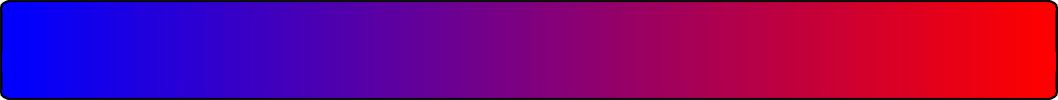
\includegraphics[width=\linewidth,height=0.05in,keepaspectratio]{../bin/colormaps/resource/pymol_blue_red_spectrum.png}};
    %
    \node(rmsdlabel) [above, inner sep=2pt] at (spectrumbarrmsd.north) {RMSD};
    %
    \node(rmsdlabelwest) [below, inner sep=6pt, align=center] at (spectrumbarrmsd.north west) {1.5 \AA};
    \node(rmsdlabeleast) [below, inner sep=6pt, align=center] at (spectrumbarrmsd.north east) {18 \AA};
    %
    \path (overlay_rmsd.north east)++(-0.25,-0.25) coordinate (arcstart);
    %
    \path[dashed edge] (dimer_roi_left.north) edge (closeup_143_rect.north west);
    \path[dashed edge] (dimer_roi_center.south) edge (closeup_310_rect.north east);
    \draw[<-, line width=0.2mm] (arcstart) arc (30:90:1);
    \node(arclabel) [below, inner sep=3pt] at (arcstart) {\ang{20}};
\end{tikzcanvas}
\end{conditionalpanel}
\begin{conditionalcaption}
\caption[The intra-dimer interface of cardiac calsequestrin]{\textbf{\headingsubsubsectionfour}. \figurepanelcaptiona Dimer with ytterbium (Yb) sites (magenta spheres) within its interior cavity. Closeups focus on Yb positions that bridge dimer chains A and B: relatively high occupancy is observed in a narrow intra-dimer cleft (right detail panel), while a site of weaker interaction and weaker occupancy is identified in the intra-dimer cavity (lower detail panel). \figurepanelcaptionb Comparison of a previously published cardiac calsequestrin dimer (1SJI) to the more tightly packed dimer that we report. The tightly packed dimer results primarily from rigid body rotation of the dimer chains inward (for a single chain, we observe \ang{20} counterclockwise rotation in the plane of the page when the other chain is fixed to the reference dimer). The inward rotation produces an increase in buried surface area (BSA) in thioredoxin domains II and III.}
\label{fig:intra_dimer_interface}
\end{conditionalcaption}
\end{figure}
\begin{figure}[!h]
\centering
%\figuretitle{Figure~\ref{fig:inter_dimer_interface}}
\begin{conditionalpanel}
    \begin{tikzcanvas}{}
    %
    %
    % Overview Yb with cutaway
    % at (current page.north)
    \node(overview)[inner sep=0pt,below right] {\includegraphics[width=\linewidth,height=2.75in,keepaspectratio]{../results/inter_dimer_interface/output/tetramer_interface_overview_yb_cropped.png}};
    %
    \path (overview.north)++(-0.4,-3.5) coordinate (ybD144SW);
    \path (overview.north)++(0.4,-3) coordinate (ybD144NE);
    \node(ybD144) [fit={(ybD144SW) (ybD144NE)}, dashedrectanglefit] {};
    %
    \path (overview.north)++(-0.4,-2.4) coordinate (ybE184SW);
    \path (overview.north)++(0.4,-1.9) coordinate (ybE184NE);
    \node(ybE184) [fit={(ybE184SW) (ybE184NE)}, dashedrectanglefit] {};
    %
    \path (overview.north)++(-0.4,-4.6) coordinate (ybD348SW);            
    \path (overview.north)++(0.4,-4.1) coordinate (ybD348NE);
    \node(ybD348) [fit={(ybD348SW) (ybD348NE)}, dashedrectanglefit] {};    
    %
    \path (overview.south)++(-0.5,1.25) coordinate (ybD351SW);            
    \path (overview.south)++(0.5,1.75) coordinate (ybD351NE);
    \node(ybD351) [fit={(ybD351SW) (ybD351NE)}, dashedrectanglefit] {};
    %
    %
    \path (overview.west)++(4.5,0.65) coordinate (cavityedge);
    \path (overview.west)++(-0.5,2.25) coordinate (cSolventCavityLabel);
    \node(solventcavitylabel) [above, inner sep=3pt, align=center, font=\footnotesize] at (cSolventCavityLabel) {Inter-Dimer\\Solvent Cavity};
    \path[-,thick] (cSolventCavityLabel.east) edge (cavityedge.south);

    \path (overview.west)++(0.25,1) coordinate (chainA);            
    \path (overview.north)++(-2.75,-0.5) coordinate (chainB);
    \path (overview.north)++(2.75,-0.5) coordinate (chainAprime);
    \path (overview.east)++(-0.25,1) coordinate (chainBprime);

    \node(chainAlabel) [above, inner sep=2pt, align=center] at (chainA) {Chain A};
    \node(chainBlabel) [above, inner sep=2pt, align=center] at (chainB) {Chain B};
    \node(chainAprimelabel) [above, inner sep=2pt, align=center] at (chainAprime) {Chain A'};
    \node(chainBprimelabel) [above, inner sep=2pt, align=center] at (chainBprime) {Chain B'};
    %
    %
    %
    \node(D348D350)[inner sep=0pt,below=0.5cm of overview]{\includegraphics[width=\linewidth,height=1.5in,keepaspectratio]{../results/inter_dimer_interface/output/tetramer_interface_D348_D350_closeup_yb_cropped.png}};
    %
    \node(closeuprectD348D350) [fit=(D348D350), dashedrectanglefit] {};
    % Label
    \node(D348D350label) [above, inner sep=5pt, align=center] at (D348D350.north) {D348/D350 Inter-Dimer Region};
    %
    \node(D348D350Rotator) at ([yshift=0.35cm]D348D350label.north) {\AxisRotator};
    \draw[line width=0.1ex] (D348D350Rotator.west) -- (D348D350Rotator.east);
    \node(D348D350RotatorLabel)[inner sep=4pt,right] at (D348D350Rotator.east) {\ang{90}};  
    % D348_B'
    \path (D348D350.north)++(1.75,-1) coordinate (cD348chainD);
    \node(D348) [above, inner sep=0pt, font=\small, font=\bfseries] at (cD348chainD) {D348};
    % D348_A
    \path (D348D350.south)++(-2,+0.75) coordinate (cD348chainA);
    \node(D348chainA) [above, inner sep=0pt, font=\small, font=\bfseries] at (cD348chainA) {D348};
    %
    % D350_B'
    \path (D348D350.south)++(2,+0.75) coordinate (cD350chainD);
    \node(D350) [above, inner sep=0pt, font=\small, font=\bfseries] at (cD350chainD) {D350};
    % D350_A
    \path (D348D350.north)++(-2,-1) coordinate (cD350chainA);
    \node(D350chainA) [above, inner sep=0pt, font=\small, font=\bfseries] at (cD350chainA) {D350};
    %
    %
    %
    %        \path (overview.west)++(-3,-0.25) coordinate (anchor_D144E174);  %
    \node(D144E174)[inner sep=0pt,left=3.5cm of D348D350.south]{\includegraphics[width=\linewidth,height=1.75in,keepaspectratio]{../results/inter_dimer_interface/output/tetramer_interface_D144_E174_closeup_yb_cropped.png}};
    %
    % rect
    \node(closeuprectD144E174) [fit=(D144E174), dashedrectanglefit] {};
    % label        
    \node(D144E174label) [above, inner sep=5pt, align=center] at (D144E174.north) {D144/E174 Inter-Dimer Region};
    %
    \node(D144E174Rotator) at ([yshift=0.35cm]D144E174label.north) {\AxisRotator};
    \draw[line width=0.1ex] (D144E174Rotator.west) -- (D144E174Rotator.east);
    \node(D144E174RotatorLabel)[inner sep=4pt,right] at (D144E174Rotator.east) {\ang{90}};  
    % D144 
    \path (D144E174.west)++(0.5,1.75)  coordinate (cD144_B);
    \path (D144E174.east)++(-0.5,-2)  coordinate (cD144_Aprime);
    \node(D144_B) [above, inner sep=0pt, font=\small, font=\bfseries] at (cD144_B) {D144};
    \node(D144_Aprime) [above, inner sep=0pt, font=\small, font=\bfseries] at (cD144_Aprime) {D144};
    % 174 
    \path (D144E174.south west)++(0.1,0.4) coordinate (cE174_B);
    \path (D144E174.north east)++(-0.1,-0.6) coordinate (cE174_Aprime);
    \node(E174_B) [above right, inner sep=0pt, font=\small, font=\bfseries] at (cE174_B) {E174};   
    \node(E174_Aprime) [below left, inner sep=0pt, font=\small, font=\bfseries] at (cE174_Aprime) {E174};   
    %
    %
    %
    \node(D351E357)[inner sep=0pt,below=3cm of D348D350.south,anchor=center]{\includegraphics[width=\linewidth,height=1.5in,keepaspectratio]{../results/inter_dimer_interface/output/tetramer_interface_D351_E357_closeup_yb_cropped.png}};
    %
    \node(closeuprectD351E357) [fit=(D351E357), dashedrectanglefit] {};
    % Label
    \node(D351E357label) [above, inner sep=5pt, align=center] at (D351E357.north) {D351/E357 Inter-Dimer Region};
    % D351
    \path (D351E357.north)++(0,-1) coordinate (cD351);
    \node(D351) [above, inner sep=0pt, font=\small, font=\bfseries] at (cD351) {D351};
    % E357
    \path (D351E357.south)++(0,+1) coordinate (cE357);
    \node(E357) [above, inner sep=0pt, font=\small, font=\bfseries] at (cE357) {E357};
    %
    \path (closeuprectD351E357.north east)++(0,5) coordinate (ybD351_waypoint);
    \path[dashed edge] (ybD348.north west) edge (closeuprectD348D350.north west);
    \path[dashed edge] (ybD351.north east) edge (ybD351_waypoint);
    \path[dashed edge] (ybD351_waypoint) edge (closeuprectD351E357.north east);
    %
    %
    \node(E184E187)[inner sep=0pt,right=3.5cm of D351E357.north]{\includegraphics[width=\linewidth,height=3.25in,keepaspectratio]{../results/inter_dimer_interface/output/tetramer_interface_E184_E187_closeup_yb_cropped.png}};
    % rect
    \node(closeuprectE184E187) [fit=(E184E187), dashedrectanglefit] {};
    % label        
    \node(E184E187label) [above, inner sep=5pt, align=center] at (E184E187.north) {D50/K180/E184/E187 Inter-Dimer Region};
    % rotator
    % \node(E184E187Rotator) at (E184E187label.north) {\AxisRotator[rotate=90]};
    \node(E184E187Rotator) at ([yshift=0.35cm]E184E187label.north) {\AxisRotator};
    \draw[line width=0.1ex] (E184E187Rotator.west) -- (E184E187Rotator.east);
    \node(E184E187RotatorLabel)[inner sep=4pt,right] at (E184E187Rotator.east) {\ang{90}};  
    % E184 
    \path (E184E187.west)++(1,1)  coordinate (cE184);
    \node(E184) [above, inner sep=0pt, font=\small, font=\bfseries] at (cE184) {E184};
    % E187 
    \path (E184E187.north)++(-1,-0.4) coordinate (cE187);
    \node(E187) [above, inner sep=0pt, font=\small, font=\bfseries] at (cE187) {E187};        
    % D50
    \path (E184E187.east)++(-1,1) coordinate (cD50);
    \node(D50) [above, inner sep=0pt, font=\small, font=\bfseries] at (cD50) {D50};
    % K180 
    \path (E184E187.north)++(1,-0.4) coordinate (cK180);
    \node(K180) [above, inner sep=0pt, font=\small, font=\bfseries] at (cK180) {K180};
    %
    % Other side.
    %
    % E184 
    \path (E184E187.east)++(-1,-1.4)  coordinate (cE184_low);
    \node(E184_low) [above, inner sep=0pt, font=\small, font=\bfseries] at (cE184_low) {E184};
    % E187 
    \path (E184E187.south)++(1,0.25) coordinate (cE187_low);
    \node(E187_low) [above, inner sep=0pt, font=\small, font=\bfseries] at (cE187_low) {E187};        
    % D50
    \path (E184E187.west)++(1,-1.4) coordinate (cD50_low);
    \node(D50_low) [above, inner sep=0pt, font=\small, font=\bfseries] at (cD50_low) {D50};
    % K180 
    \path (E184E187.south)++(-1.5,0.25) coordinate (cK180_low);
    \node(K180_low) [above, inner sep=0pt, font=\small, font=\bfseries] at (cK180_low) {K180};
    %
    %
    \path[dashed edge] (ybD144.north west) edge (closeuprectD144E174.north west);
    \path[dashed edge] (ybE184.north east) edge (closeuprectE184E187.north east);
    %
%        \path (D144E174.west)++(-0.5,0) coordinate (D144A_E174A_plot_anchor);
    %
    \node(D144A_E174A_plot)[inner sep=0pt,anchor=west] at ([xshift=-0.75cm,yshift=-8cm]D144E174.west){\input{../results/assembly_kinetics/output/kinetics_interface_mutation_D144A_E174A_85mM_K.pgf}};
    %
    \node(E184A_E187A_plot)[inner sep=0pt,right=0.25cm of D144A_E174A_plot]{\input{../results/assembly_kinetics/output/kinetics_interface_mutation_E184A_E187A_85mM_K.pgf}};
    %
    \node(D50A_plot)[inner sep=0pt,right=0.25cm of E184A_E187A_plot]{\input{../results/assembly_kinetics/output/kinetics_interface_mutation_D50A_85mM_K.pgf}};
    %
    \node(captionB)[inner sep=10pt,above right] at (D144A_E174A_plot.north west) {\normalsize\textbf{\figurepanelb}};
    %
    \node(captionA)[inner sep=10pt,below right] at ([shift={(0cm,18cm)}]D144A_E174A_plot.north west) {\normalsize\textbf{\figurepanela}};
\end{tikzcanvas}
\end{conditionalpanel}
\begin{conditionalcaption}
\caption[The inter-dimer interface of cardiac calsequestrin]{\textbf{\headingsubsubsectionfive}. \figurepanelcaptiona Yb (magenta spheres) bound within the walled pocket formed by the inter-dimer interface, with closeups of ytterbium sites at D144 and E174, E184 and E187, D348 and D350, and D351 and D357. Thioredoxin domain II of chain A' (blue) is omitted to allow visualization of the interior of the solvent pocket formed by the inter-dimer interface. \figurepanelcaptionb Turbidity assays after alanine mutagenesis of putative calcium-binding and salt bridge residues. Left: D144A and E174A. Middle: E184A and E187A. Right: D50A. All graphed values are mean of 3 technical replicates ± SD.}
\label{fig:inter_dimer_interface}
\end{conditionalcaption}
\end{figure}
\begin{figure}[!h]
\centering
%\figuretitle{Figure~\ref{fig:filament_cavity}}
\begin{conditionalpanel}
    \begin{tikzcanvas}{}
    %
    \node(axialdimer)[inner sep=0pt,below right]{\includegraphics[width=\linewidth,height=1.25in,keepaspectratio]{../results/cavity/output/dimer_cavity_axial_cropped.png}};
    %
    \path (axialdimer.north)++(-0.25,-1.35) coordinate (axialdimerROISW1);           
    \path (axialdimer.north)++(0.25,-2.1) coordinate (axialdimerROINE1);
    \node(axialdimerROIrect) [fit={(axialdimerROISW1) (axialdimerROINE1)}, dashedrectanglefit] {};
    %
    \node(captionA)[inner sep=0pt,above left] at (axialdimer.north west) {\normalsize\textbf{\figurepanela}};
    %
    \path (axialdimer.south west)++(0.4,-0.5) coordinate (chainArotated);           
    \path (axialdimer.south east)++(-0.4,-0.5) coordinate (chainBrotated);
    %
    \node(chainArotatedlabel) [above, inner sep=2pt, align=center] at (chainArotated) {Chain A};
    \node(chainBrotatedlabel) [above, inner sep=2pt, align=center] at (chainBrotated) {Chain B};
    %
    %
    %
    \node(axialdimerapbs)[inner sep=0pt,right=0.5cm of axialdimer]{\includegraphics[width=\linewidth,height=1.25in,keepaspectratio]{../results/cavity/output/dimer_cavity_apbs_axial_no_ramp_cropped.png}};
    %
    \node(axialdimerlabel) [below, inner sep=2pt, align=center] at (axialdimerapbs.south) {Solvent-Exposed Side\\(Filament End Cap)};
    %
    \path (axialdimerapbs.north)++(-0.25,-1.35) coordinate (axialdimerapbsROISW1);   
    \path (axialdimerapbs.north)++(0.25,-2.1) coordinate (axialdimerapbsROINE1);
    \node(axialdimerapbsROIrect) [fit={(axialdimerapbsROISW1) (axialdimerapbsROINE1)}, dashedrectanglefit] {};
    %
    \path[dashed edge] (axialdimerROIrect.east) edge (axialdimerapbsROIrect.west);
    %
    %
    %
    \node(spectrumbar)[inner sep=0pt,right=0.5cm of axialdimerapbs.east]{\rotatebox[origin=c]{-90}{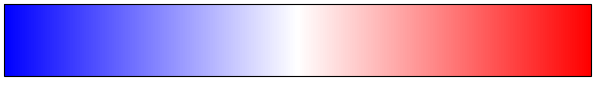
\includegraphics[width=\linewidth,height=0.15in,keepaspectratio]{../bin/colormaps/resource/matplotlib_bwr.png}}};
    %
    \node(apbslabel) [above, inner sep=6pt] at (spectrumbar.north) {30 kT/e};
    \node(apbslabel) [below, inner sep=6pt] at (spectrumbar.south) {-30 kT/e};       
    %
    %
    %
    \node(tetramer)[inner sep=0pt,right=2cm of spectrumbar.east]{\includegraphics[width=\linewidth,height=1.25in,keepaspectratio]{../results/cavity/output/tetramer_cavity_apbs_side_no_ramp_cropped.png}};
    %
    \node(captionB)[inner sep=0pt,above left] at (tetramer.north west) {\normalsize\textbf{\figurepanelb}};
    %
    \path (tetramer.north)++(-0.5,-0.95) coordinate (tetramerROISW1);            
    \path (tetramer.north)++(0.5,-1.8) coordinate (tetramerROINE1);
    \node(tetramerROIrect) [fit={(tetramerROISW1) (tetramerROINE1)}, dashedrectanglefit] {};
    %
    %
    \path (tetramer.west)++(-0.25,0.5) coordinate (chainA_tetramer);           
    \path (tetramer.north)++(-1.5,0) coordinate (chainB_tetramer);
    \path (tetramer.north)++(1.5,0) coordinate (chainAprime_tetramer);
    \path (tetramer.east)++(0.25,0.5) coordinate (chainBprime_tetramer);
    %
    \node(chainAlabel) [above, inner sep=2pt, align=center] at (chainA_tetramer) {Chain A};
    \node(chainBlabel) [above, inner sep=2pt, align=center] at (chainB_tetramer) {Chain B};
    \node(chainAprimelabel) [above, inner sep=2pt, align=center] at (chainAprime_tetramer) {Chain A'};
    \node(chainBprimelabel) [above, inner sep=2pt, align=center] at (chainBprime_tetramer) {Chain B'};
    %
    \node(D144_E174_closeup)[inner sep=0pt,below=1cm of tetramer.south,anchor=north]{\includegraphics[width=\linewidth,height=1.5in,keepaspectratio]{../results/cavity/output/tetramer_cavity_D144_E174_closeup_no_ramp_cropped.png}};
    %
    \node(closeuprectD144E174) [fit=(D144_E174_closeup), dashedrectanglefit] {};
    %
    \path[dashed edge] (tetramerROIrect.south) edge (closeuprectD144E174.north);
    %
    \path (D144_E174_closeup.south west)++(0.5,-0.65) coordinate (cE174label);
    \path (D144_E174_closeup.west)++(1.125,-0.65) coordinate (cE174);
    \node(E174) [above, inner sep=3pt, font=\small, font=\bfseries] at (cE174label) {E174};
    \path[-,thick] (E174.north) edge (cE174.south);
    %
    \path (D144_E174_closeup.south east)++(-0.5,-0.65) coordinate (cD144label);
    \path (D144_E174_closeup.east)++(-1.125,-0.3) coordinate (cD144);
    \node(D144) [above, inner sep=3pt, font=\small, font=\bfseries] at (cD144label) {D144};
    \path[-,thick] (D144.north) edge (cD144.south);
    %
    \node(filament)[inner sep=0pt,below=4.5cm of axialdimer.west,anchor=west]{\includegraphics[width=\linewidth,height=1.25in,keepaspectratio]{../results/cavity/output/filament_cavity_and_yb_blend_cutaway_cropped.png}};
    %
    \node(captionC)[inner sep=0pt,above left] at (filament.north west) {\normalsize\textbf{\figurepanelc}};
    %
\end{tikzcanvas}
\end{conditionalpanel}
\begin{conditionalcaption}
\caption[The electronegative lumen within the cardiac calsequestrin filament]{\textbf{\headingsubsectionsix}. \figurepanelcaptiona Left panel: the interior cavity of the dimer viewed down its long axis. Residues that interact with Yb atoms within the intra-dimer cleft (\maintextfigure~\ref{fig:intra_dimer_interface}) are shown as sticks. All other residues are rendered as surface. Right side: APBS-generated electrostatic surface of the same region. \figurepanelcaptionb The lumen is continuous down the length of filament because of the large solvent cavity formed at each dimer-dimer interface. The APBS-generated electrostatic surface of the lumen (as traced by HOLLOW using a 1.4 \AA\ probe) is shown, with closeup of residues D144 and E174 deep within the electronegative cavity. \figurepanelcaptionc View of the filament and its continuous interior cavity, with Yb sites shown as magenta spheres.}
\label{fig:filament_cavity}
\end{conditionalcaption}
\end{figure}
\begin{figure}[!h]
\centering
%\figuretitle{Figure~\ref{fig:inter_dimer_interface_cpvt}}
\begin{conditionalpanel}
    \begin{tikzcanvas}{}
        \node(overview1)[inner sep=0pt,below right]{\includegraphics[width=\linewidth,height=1.75in,keepaspectratio]{../results/inter_dimer_interface/output/tetramer_interface_overview_CPVT_cropped.png}};
        %
        \path (overview1.north)++(-1,-2.5) coordinate (S173SW1);            
        \path (overview1.north)++(-0.375,-1.75) coordinate (S173NE1);
        \node(S173one) [fit={(S173SW1) (S173NE1)}, dashedrectanglefit] {};
        %
        \path (overview1.north)++(0.375,-2.5) coordinate (S173SW2);           
        \path (overview1.north)++(1,-1.75) coordinate (S173NE2);
        \node(S173two) [fit={(S173SW2) (S173NE2)}, dashedrectanglefit] {};
        %
        %
        \path (overview1.north)++(-0.5,-1.75) coordinate (K180SW1);            
        \path (overview1.north)++(0,-1.125) coordinate (K180NE1);
        \node(K180one) [fit={(K180SW1) (K180NE1)}, dashedrectanglefit] {};
        %
        \path (overview1.north)++(0,-1.75) coordinate (K180SW2);           
        \path (overview1.north)++(0.5,-1.125) coordinate (K180NE2);
        \node(K180two) [fit={(K180SW2) (K180NE2)}, dashedrectanglefit] {};
        %
        \path (overview1.west)++(0,1) coordinate (chainA);           
        \path (overview1.north)++(-2.4,-0.5) coordinate (chainB);
        \path (overview1.north)++(2.4,-0.5) coordinate (chainAprime);
        \path (overview1.east)++(-0.25,1) coordinate (chainBprime);

        \node(chainAlabel) [above, inner sep=2pt, align=center] at (chainA) {Chain A};
        \node(chainBlabel) [above, inner sep=2pt, align=center] at (chainB) {Chain B};
        \node(chainAprimelabel) [above, inner sep=2pt, align=center] at (chainAprime) {Chain A'};
        \node(chainBprimelabel) [above, inner sep=2pt, align=center] at (chainBprime) {Chain B'};
        %
        %
        %
        \node(closeup180)[inner sep=0pt,below right,right=1.5cm of overview1]{\includegraphics[width=\linewidth,height=1.5in,keepaspectratio]{../results/inter_dimer_interface/output/tetramer_interface_K180_closeup_yb_cropped.png}};
        \node(closeup180rect) [fit=(closeup180), dashedrectanglefit] {};
        %
        \node(K180_ROI_label) [above, inner sep=5pt, align=center] at (closeup180.north) {D50/K180/E184/E187 Inter-Dimer Region};
        %
        \node(K180Rotator) at ([yshift=-1cm]K180_ROI_label.north) {\AxisRotator};
        \draw[line width=0.1ex] (K180Rotator.west) -- (K180Rotator.east);
        \node(K180RotatorLabel)[inner sep=4pt,right] at (K180Rotator.east) {\ang{60}};  
        %
        % E184 
        \path (closeup180.east)++(-1,-1.4)  coordinate (cE184);
        \node(E184_label) [above, inner sep=0pt, font=\small, font=\bfseries] at (cE184) {E184};
        % E187 
        \path (closeup180.east)++(-0.4,0.4) coordinate (cE187);
        \node(E187_label) [above, inner sep=0pt, font=\small, font=\bfseries] at (cE187) {E187};
        % D50
        \path (closeup180.west)++(0.75,0.4) coordinate (cD50);
        \node(D50_label) [above, inner sep=0pt, font=\small, font=\bfseries] at (cD50) {D50};
        % K180 
        \path (closeup180.west)++(2.2,0.3) coordinate (cK180);
        \node(K180) [above, inner sep=0pt, font=\small, font=\bfseries] at (cK180) {K180};
        %
        \path[dashed edge] (K180two.north east) edge (closeup180rect.north west);
        %
        %
        %
        \node(closeup173)[inner sep=0pt,below=3.5cm of overview1.south west,anchor=west]{\includegraphics[width=\linewidth,height=1.5in,keepaspectratio]{../results/inter_dimer_interface/output/tetramer_interface_S173_closeup_cropped.png}};
        \node(closeup173rect) [fit=(closeup173), dashedrectanglefit] {};
        %
        \node(S173_ROI_label) [above, inner sep=5pt, align=center] at (closeup173.north) {K87/S173/D325 Inter-Dimer Region};
        % S173
        \path (closeup173.west)++(1.5,0.25) coordinate (cS173);
        \node(S173) [above, inner sep=0pt, font=\small, font=\bfseries] at (cS173) {S173};
        % D325
        \path (closeup173.south)++(-1.25,+0.25) coordinate (cD325);
        \node(D325) [above, inner sep=0pt, font=\small, font=\bfseries] at (cD325) {D325}; 
        % D319
        \path (closeup173.south)++(2,1) coordinate (cD319);
        \node(D319) [above, inner sep=0pt, font=\small, font=\bfseries] at (cD319) {D319}; 
        % K87
        \path (closeup173.east)++(-1.25,0.5) coordinate (cK87);
        \node(K87) [above, inner sep=0pt, font=\small, font=\bfseries] at (cK87) {K87}; 
        % K172
        \path (closeup173.west)++(2.5,-0.4) coordinate (cK172);
        \node(K87) [above, inner sep=0pt, opacity=.4, font=\footnotesize, font=\bfseries] at (cK172) {K172}; 
        %
        \path[dashed edge] (S173one.south west) edge (closeup173rect.north west);
        %
        %
        %
        \node(D325A_plot)[inner sep=0pt,right=1.5cm of closeup173.east,anchor=west]{\input{../results/assembly_kinetics/output/kinetics_interface_mutation_D325A_D325I_85mM_K.pgf}};
        %
%        \node(closeuprectD325Aplot) [fit=(D325A_plot), dashedrectanglefit] {};
        %
%        \path[dashed edge] (closeup173rect.east) edge (closeuprectD325Aplot.west);
        %
        \node(captionA)[inner sep=10pt,above left] at (overview1.north west) {\normalsize\textbf{\figurepanela}};
        %
        \node(captionB)[inner sep=10pt,above left] at ([xshift=9cm]overview1.north west) {\normalsize\textbf{\figurepanelb}};
        %
        \node(captionC)[inner sep=10pt,above left] at (closeup173.north west) {\normalsize\textbf{\figurepanelc}};
        %
        \node(captionD)[inner sep=10pt,above left] at ([xshift=7cm]closeup173.north west) {\normalsize\textbf{\figurepaneld}};
    \end{tikzcanvas}
\end{conditionalpanel}
\begin{conditionalcaption}
\caption[The S173 and K180 residues are at the cardiac calsequestrin inter-dimer interface]{\textbf{\headingsubsectionseven}. \figurepanelcaptiona Inter-dimer interface residues in the vicinity of S173 and K180 shown as spheres. \figurepanelcaptionb Closeup of K180 with the adjacent E184 and E187 cation binding site, with the coordinated Yb atom shown as a sphere. \figurepanelcaptionc Hydrophilic pocket at S173. In this pocket, 3 different thioredoxin domains from 3 distinct chains interact (K87, S173, D325). K172 (backgrounded) is the most proximal of several residues that shield the pocket from bulk solvent. \figurepanelcaptiond Turbidity assay with the D325A and D325I mutations. All graphed values are mean of 3 technical replicates ± SD.}
\label{fig:inter_dimer_interface_cpvt}
\end{conditionalcaption}
\end{figure}
\begin{figure}[!h]
\centering
%\figuretitle{Figure~\ref{fig:graphical_summary}}
\begin{conditionalpanel}
    % All about specifying coords: https://stuff.mit.edu/afs/athena/contrib/tex-contrib/beamer/pgf-1.01/doc/generic/pgf/version-for-tex4ht/en/pgfmanualse8.html
    \tikzset{
        monomerA/.pic = {
            \draw[fill=orange,rounded corners] (-0.5,0)  
            -- ++(0.75,0) 
            -- ++(0.5,-1) 
            -- ++(-1.25,0) 
            -- cycle;
        }
    }
    \tikzset{
        monomerAmutantIntra/.pic = {
            \draw[fill=red,rounded corners] (-0.5,0) node(monomerAanchor)[inner sep=14] {}
            -- ++(0.75,0) 
            -- ++(0.5,-1) 
            -- ++(-1.25,0) 
            -- cycle;
            \draw[fill=LimeGreen,rounded corners] (-0.5,0) node(monomerAanchor2)[inner sep=14] {} 
            -- ++(0.625,0) 
            -- ++(0.5,-1) 
            -- ++(-1.125,0) 
            -- cycle;
            % Was previously using a start to indicate the mutant.
            % \node[star,star points=5, draw, fill=red,star point ratio=2.25,inner sep=0pt,minimum height=0.5cm] at ([xshift=-0.05cm]monomerAanchor.south east) {};
        }
    }
    \tikzset{
        monomerAmutantInter/.pic = {
            \draw[fill=red,rounded corners] (-0.5,0) node(monomerAanchor)[inner sep=14] {}
            -- ++(0.75,0) 
            -- ++(0.5,-1) 
            -- ++(-1.25,0) 
            -- cycle;
            \draw[fill=LimeGreen,rounded corners] (-0.375,0) node(monomerAanchor2)[inner sep=14] {} 
            -- ++(0.625,0) 
            -- ++(0.5,-1) 
            -- ++(-1.125,0) 
            -- cycle;
        }
    }
    % "B" chain
    \tikzset{
        monomerB/.pic = {
            \draw[fill=orange,rounded corners] (-0.5,0)  
            -- ++(1.25,0) 
            -- ++(0,-1) 
            -- ++(-0.75,0) 
            -- cycle;
        }
    }
    \tikzset{
        monomerBmutantIntra/.pic = {
            \draw[fill=red,rounded corners] (-0.5,0) node(monomerBanchor)[inner sep=14] {}
            -- ++(1.25,0) 
            -- ++(0,-1) 
            -- ++(-0.75,0) 
            -- cycle;
            \draw[fill=LimeGreen,rounded corners] (-0.375,0) node(monomerBanchor)[inner sep=14] {} 
            -- ++(1.125,0) 
            -- ++(0,-1) 
            -- ++(-0.625,0) 
            -- cycle;
        }
    }
    \tikzset{
        monomerBmutantInter/.pic = {
            \draw[fill=red,rounded corners] (-0.5,0) node(monomerBanchor)[inner sep=14] {}
            -- ++(1.25,0) 
            -- ++(0,-1) 
            -- ++(-0.75,0) 
            -- cycle;
            \draw[fill=LimeGreen,rounded corners] (-0.5,0) node(monomerBanchor)[inner sep=14] {} 
            -- ++(1.125,0) 
            -- ++(0,-1) 
            -- ++(-0.625,0) 
            -- cycle;
        }
    }
%     \begin{tikzcanvas}{}
%         % https://tex.stackexchange.com/questions/185279/anchoring-tikz-pics
%         %
%         \node(legendTitle)[align=center,font=\small,font=\bfseries, minimum size=2cm] at (current page.north) {Heterozygous Missense Genotypes};
%         \node(legendCenter)[align=center,below=0.125cm of legendTitle.south] {};
%         %
% %        \pic at ([xshift=-0.45cm,yshift=-0.6cm]legendWT.north) {monomerA};
% %        \pic at ([xshift=0.45cm,yshift=-0.6cm]legendWT.north) {monomerB};
%         %
%         \node(legendIntra)[left=1cm of legendCenter.west,align=center] {\textit{Intra}-Dimer Mutant};
%         %
%         \pic at ([xshift=-1cm,yshift=-0.6cm]legendIntra.north) {monomerA};
%         \node(X1)[align=center,color=red,font=\bfseries, font=\large, minimum size=2cm] at ([xshift=0cm,yshift=-0.7cm]legendIntra.south) {\Large \bf X};
%         \pic at ([xshift=0.75cm,yshift=-0.6cm]legendIntra.north) {monomerBmutantIntra};
%         %
%         \node(legendInter)[right=1cm of legendCenter.east,align=center] {\textit{Inter}-Dimer Mutant};
%         %
%         \pic at ([xshift=-0.45cm,yshift=-0.6cm]legendInter.north) {monomerA};
%         \pic at ([xshift=0.45cm,yshift=-0.6cm]legendInter.north) {monomerBmutantInter};
%         %
%         \draw[thick] ($(legendIntra.north west)+(-1,0.5)$) rectangle ($(legendInter.south east)+(1,-1.75)$);
%     \end{tikzcanvas}
%     \vspace{0.75cm}
    \begin{tikzcanvas}{}
        \node(genotypesLabel)[below right,align=center,font=\small,font=\bfseries] {Genotype};
        %
%        \node(chainTypesLabel)[right=2cm of genotypesLabel.east,align=center,font=\small,font=\bfseries, minimum size=2cm] {Protomers};
        %
        \node(retainedLabel)[right=0.9cm of genotypesLabel.east,align=center,font=\small,font=\bfseries] {Retained};
        % 
        \node(traffickedLabel)[right=1.7cm of retainedLabel.east,align=center,font=\small,font=\bfseries] {Exported};
        %
        % First separator
        %
        \path (genotypesLabel.south)++(-1,-0.25) coordinate (Separator1Left);
        \path (traffickedLabel.south)++(1.55,-0.25) coordinate (Separator1Right);
        \path[-] (Separator1Left) edge (Separator1Right);
        %
        %
        \node(hetIntraLabel)[below=1cm of genotypesLabel.south,align=center,font=\footnotesize] {Heterozygous\\\textit{Intra}-Dimer\\Mutant};
        %
        % \node(IntraChainTypes)[below=1cm of chainTypesLabel.south,align=center] {};
        % %
        % \pic at ([xshift=-0.75cm]IntraChainTypes.north) {monomerA};
        % \pic at ([xshift=0.75cm]IntraChainTypes.south) {monomerBmutantIntra};
        %
        \node(hetIntraHomoWT)[below=1cm of retainedLabel.south,align=center] {};
        %
        \pic at ([xshift=-0.45cm]hetIntraHomoWT.north) {monomerA};
        \pic at ([xshift=0.45cm]hetIntraHomoWT.north) {monomerB};
        \node(retainedPctIntra)[below=1cm of hetIntraHomoWT.south,align=center,font=\bfseries,font=\footnotesize] {\SI{50}{\percent}};
        %
        \node(hetIntraHomoMut)[align=center] at ([xshift=-0.2cm,yshift=-1.1cm]traffickedLabel.south) {};
        %
        \pic at ([xshift=-0.55cm]hetIntraHomoMut.north) {monomerAmutantIntra};
        \node(X2)[align=center,color=red,font=\large,font=\bfseries, minimum size=2cm] at ([xshift=0.3cm,yshift=-0.3cm]hetIntraHomoMut.south) {\normalsize \bf X};
        \pic at ([xshift=0.85cm]hetIntraHomoMut.north) {monomerBmutantIntra};
        %
        %
        %
        \path (genotypesLabel.south)++(-1,-3) coordinate (separator2Left);
        \path (traffickedLabel.south)++(1.55,-3) coordinate (separator2Right);
        \path[-] (separator2Left) edge (separator2Right);
        %
        %
        %
        \node(hetInterLabel)[below=3.5cm of genotypesLabel.south,align=center,font=\footnotesize] {Heterozygous\\\textit{Inter}-Dimer\\Mutant};
        %
        % \node(hetInterChainTypes)[below=3.5cm of chainTypesLabel.south,align=center] {};
        % %
        % \pic at ([xshift=-0.75cm]hetInterChainTypes.north) {monomerA};
        % \pic at ([xshift=0.75cm]hetInterChainTypes.south) {monomerBmutantInter};
        %
        % Retained
        %
        \node(hetInterHomoWT)[below=3.5cm of retainedLabel.south,align=center] {};
        %
        \pic at ([xshift=-0.45cm]hetInterHomoWT.north) {monomerA};
        \pic at ([xshift=0.45cm]hetInterHomoWT.north) {monomerB};
        \node(retainedPctInter)[below=1cm of hetInterHomoWT.south,align=center,font=\bfseries,font=\footnotesize] {\SI{25}{\percent}};
        %
        % Exported
        %
        \node(hetInterHet1)[below=3.5cm of traffickedLabel.south,align=center] {};
        %
        \pic at ([xshift=-0.45cm]hetInterHet1.north) {monomerA};
        \pic at ([xshift=0.45cm]hetInterHet1.north) {monomerBmutantInter};

        \node(hetInterHet2)[below=1.25cm of hetInterHet1.south,align=center] {};

        \pic at ([xshift=-0.45cm]hetInterHet2.north) {monomerAmutantInter};
        \pic at ([xshift=0.45cm]hetInterHet2.north) {monomerB};

        \node(hetInterHomoMut)[below=1.25cm of hetInterHet2.south,align=center] {};

        \pic at ([xshift=-0.45cm]hetInterHomoMut.north) {monomerAmutantInter};
        \pic at ([xshift=0.45cm]hetInterHomoMut.north) {monomerBmutantInter};
        %
        %
        %
        %
        % https://tex.stackexchange.com/questions/185279/anchoring-tikz-pics
        %
        \node(legendTitle)[align=center,font=\small,font=\bfseries, minimum size=2cm] at ([xshift=0.6cm,yshift=3.5cm]retainedLabel.north) {Heterozygous Missense Genotypes};
        \node(legendCenter)[align=center,below=0.125cm of legendTitle.south] {};
        %
%        \pic at ([xshift=-0.45cm,yshift=-0.6cm]legendWT.north) {monomerA};
%        \pic at ([xshift=0.45cm,yshift=-0.6cm]legendWT.north) {monomerB};
        %
        \node(legendIntra)[left=1cm of legendCenter.west,align=center] {\textit{Intra}-Dimer Mutant};
        %
        \pic at ([xshift=-0.55cm,yshift=-0.6cm]legendIntra.north) {monomerA};
        \node(X1)[align=center,color=red,font=\bfseries, font=\large, minimum size=2cm] at ([xshift=0.3cm,yshift=-0.7cm]legendIntra.south) {\normalsize \bf X};
        \pic at ([xshift=0.85cm,yshift=-0.6cm]legendIntra.north) {monomerBmutantIntra};
        %
        \node(legendInter)[right=1cm of legendCenter.east,align=center] {\textit{Inter}-Dimer Mutant};
        %
        \pic at ([xshift=-0.45cm,yshift=-0.6cm]legendInter.north) {monomerA};
        \pic at ([xshift=0.45cm,yshift=-0.6cm]legendInter.north) {monomerBmutantInter};
        %
        \draw[thick] ($(legendIntra.north west)+(-1,0.5)$) rectangle ($(legendInter.south east)+(1,-1.75)$);
    \end{tikzcanvas}
\end{conditionalpanel}
\begin{conditionalcaption}
\caption[Disease inheritance patterns differ by location of mutation]{\textbf{Heterozygously-carried mutations at different calsequestrin interfaces have different disease inheritance patterns.} Mutations that inhibit dimerization are likely to cause penetrant disease only when carried recessively - a consequence of export of mutant monomers from the SR. However, mutations that inhibit \textit{inter}-dimer interaction are likely to have dominant effect - a consequence of the fact that only \SI{25}{\percent} of dimers remain functional for the purpose of filamentation.}
\label{fig:graphical_summary}
\end{conditionalcaption}
\end{figure}

\clearpage % help to get the table onto a new page
\section{} % Tables
\setcounter{table}{0}
\renewcommand{\thetable}{\arabic{table}}
\begin{table}[hp]
\footnotesize
\caption[Crystallographic Data Collection and Refinement]{\textbf{Crystallographic Data Collection and Refinement}}
\label{tab:table_xtal_stats}
\begin{table}[hp]
\footnotesize
\caption[Crystallographic Data Collection and Refinement]{\textbf{Crystallographic Data Collection and Refinement}}
\label{tab:table_xtal_stats}
\begin{table}[hp]
\footnotesize
\caption[Crystallographic Data Collection and Refinement]{\textbf{Crystallographic Data Collection and Refinement}}
\label{tab:table_xtal_stats}
\input{../results/table_one/output/table_xtal_stats.tex}
\end{table}

\end{table}

\end{table}

\clearpage % help to get the extended data onto a new page
\section{} % Extended Data Figures
\setcounter{figure}{0}
\setcounter{table}{0}
\renewcommand{\figurename}{Extended Data Fig.}
\renewcommand{\tablename}{Extended Data Table}
\renewcommand{\thefigure}{\arabic{figure}}
\renewcommand{\thetable}{\arabic{table}}
\begin{figure}[!h]
\centering
%\figuretitle{Figure~\ref{fig:biochemistry_supplement}}
\begin{conditionalpanel}
    \begin{tikzcanvas}{}
        \node(WT_EDTA_plot)[inner sep=0pt,above right]{\input{../results/assembly_kinetics/output/kinetics_WT_EDTA.pgf}};
        %
        \node(captionA)[inner sep=0pt,above left] at (WT_EDTA_plot.north west) {\normalsize\textbf{\figurepanela}};
        %
        \node(S173I_No_K_plot)[inner sep=0pt,right=1.25cm of WT_EDTA_plot.east, anchor=west]{\input{../results/assembly_kinetics/output/kinetics_CPVT_mutation_S173I_0mM_K.pgf}};
        %
        \node(captionB)[inner sep=0pt,above left] at (S173I_No_K_plot.north west) {\normalsize\textbf{\figurepanelb}};
        %
    \end{tikzcanvas}
\end{conditionalpanel}
\begin{conditionalcaption}
\caption[Multimerization kinetics of the S173I mutant observed in 0 mM KCl]{\textbf{Turbidity assay controls; related to \maintextfigure~\ref{fig:S173I_genetics_and_biochemistry}.} \figurepanelcaptiona Stoichiometric addition of EDTA demonstrates immediate reversal of calcium-induced turbidity. \figurepanelcaptionb Turbidity assay for the S173I mutant in \SI{0}{\milli\Molar} KCl. All graphed values are mean of 3 technical replicates ± SD.}
\label{fig:biochemistry_extended}
\end{conditionalcaption}
\end{figure}
\begin{figure}[!h]
\centering
\newcommand{\tetramerheight}{1.125in}
%\figuretitle{Figure~\ref{fig:inter_dimer_interface_BSA_comparison}}
\begin{conditionalpanel}
    \begin{tikzcanvas}{}
        \node(deo_native)[inner sep=0pt, below right] {\includegraphics[width=\linewidth,height=\tetramerheight,keepaspectratio]{../results/inter_dimer_comparison/output/tetramer_deo_native_oriented_cropped.png}};
        %
        \node (deo_native_table) [inner sep=10pt,anchor=north] at (deo_native.south) {
            \begin{tabular}{c c}
                Interface Chains & BSA (\AA\textsuperscript{2}) \\
                \hline
                \input{../results/inter_dimer_comparison/output/table_interface_comparison_tetramer_deo_native.tex}
                % B, A’ & 734.0 \\
                % A, A’ & 382.0 \\
                % B, B’ & 381.0 \\
                % A, B’ & 101.0
            \end{tabular}
        };
        %
        \node(6OVW_label) [above, inner sep=3pt, align=center] at (deo_native.north) {6OVW (This Study)\\Similar: 6OWW};
        %
        \node(1a8y)[inner sep=0pt,right=0.8cm of deo_native] {\includegraphics[width=\linewidth,height=\tetramerheight,keepaspectratio]{../results/inter_dimer_comparison/output/tetramer_1a8y_oriented_cropped.png}};
        %
        \node(1a8y_label) [above, inner sep=3pt, align=center] at (1a8y.north) {1A8Y\\Similar: 3TRP, 3TRQ, 3US3, 3V1W, 5CRD, 5KN0, 5KN3};
        %
        \node (1a8y_table) [inner sep=10pt,anchor=north] at (1a8y.south) {
            \begin{tabular}{c c}
                Interface Chains & BSA (\AA\textsuperscript{2}) \\
                \hline
                \input{../results/inter_dimer_comparison/output/table_interface_comparison_tetramer_1a8y.tex}
            \end{tabular}
        };
        %
        \node(1sji)[inner sep=0pt,right=0.8cm of 1a8y] {\includegraphics[width=\linewidth,height=\tetramerheight,keepaspectratio]{../results/inter_dimer_comparison/output/tetramer_1sji_oriented_cropped.png}};
        %
        \node(1sji_label) [above, inner sep=3pt, align=center] at (1sji.north) {1SJI};
        %
        \node (1sji_table) [inner sep=10pt,anchor=north] at (1sji.south) {
            \begin{tabular}{c c}
                Interface Chains & BSA (\AA\textsuperscript{2}) \\
                \hline
                \input{../results/inter_dimer_comparison/output/table_interface_comparison_tetramer_1sji.tex}
            \end{tabular}
        };
        %
        %
        %
        \node(2vaf)[inner sep=0pt,below=7cm of deo_native.west,anchor=west] {\includegraphics[width=\linewidth,height=\tetramerheight,keepaspectratio]{../results/inter_dimer_comparison/output/tetramer_2vaf_oriented_cropped.png}};
        %
        \node(2vaf_label) [above, inner sep=3pt, align=center] at (2vaf.north) {2VAF};
        %
        \node (2vaf_table) [inner sep=10pt,anchor=north] at (2vaf.south) {
            \begin{tabular}{c c}
                Interface Chains & BSA (\AA\textsuperscript{2}) \\
                \hline
                \input{../results/inter_dimer_comparison/output/table_interface_comparison_tetramer_2vaf.tex}
            \end{tabular}
        };
        %
        \node(3uom)[inner sep=0pt,below=7cm of 1a8y.west,anchor=west] {\includegraphics[width=\linewidth,height=\tetramerheight,keepaspectratio]{../results/inter_dimer_comparison/output/tetramer_3uom_oriented_cropped.png}};
        %
        \node(3uom_label) [above, inner sep=3pt, align=center] at (3uom.north) {3UOM};
        %
        \node (3uom_table) [inner sep=10pt,anchor=north] at (3uom.south) {
            \begin{tabular}{c c}
                Interface Chains & BSA (\AA\textsuperscript{2}) \\
                \hline
                \input{../results/inter_dimer_comparison/output/table_interface_comparison_tetramer_3uom.tex}
            \end{tabular}
        };
        %
        \node(5cre)[inner sep=0pt,below=7cm of 1sji.west,anchor=west] {\includegraphics[width=\linewidth,height=\tetramerheight,keepaspectratio]{../results/inter_dimer_comparison/output/tetramer_5cre_oriented_cropped.png}};
        %
        \node(5cre_label) [above, inner sep=3pt, align=center] at (5cre.north) {5CRE};
        %
        \node (5cre_table) [inner sep=10pt,anchor=north] at (5cre.south) {
            \begin{tabular}{c c}
                Interface Chains & BSA (\AA\textsuperscript{2}) \\
                \hline
                \input{../results/inter_dimer_comparison/output/table_interface_comparison_tetramer_5cre.tex}
            \end{tabular}
        };
        %
        %
        %
        \node(5crg)[inner sep=0pt,below=7cm of 2vaf.west,anchor=west] {\includegraphics[width=\linewidth,height=\tetramerheight,keepaspectratio]{../results/inter_dimer_comparison/output/tetramer_5crg_oriented_cropped.png}};
        %
        \node(5crg_label) [above, inner sep=3pt, align=center] at (5crg.north) {5CRG\\Similar: 5CRH};
        %
        \node (5crg_table) [inner sep=10pt,anchor=north] at (5crg.south) {
            \begin{tabular}{c c}
                Interface Chains & BSA (\AA\textsuperscript{2}) \\
                \hline
                \input{../results/inter_dimer_comparison/output/table_interface_comparison_tetramer_5crg.tex}
            \end{tabular}
        };
        %
        \node(5kn1)[inner sep=0pt,below=7cm of 3uom.west,anchor=west] {\includegraphics[width=\linewidth,height=\tetramerheight,keepaspectratio]{../results/inter_dimer_comparison/output/tetramer_5kn1_oriented_cropped.png}};
        %
        \node(5kn1_label) [above, inner sep=3pt, align=center] at (5kn1.north) {5KN1\\Similar: 5KN2};
        %
        \node (5kn1_table) [inner sep=10pt,anchor=north] at (5kn1.south) {
            \begin{tabular}{c c}
                Interface Chains & BSA (\AA\textsuperscript{2}) \\
                \hline
                \input{../results/inter_dimer_comparison/output/table_interface_comparison_tetramer_5kn1.tex}
            \end{tabular}
        };
        %
    \end{tikzcanvas}
\end{conditionalpanel}
\begin{conditionalcaption}
\caption[Comparison of buried surface area (BSA) at putative dimer-dimer multimerization interfaces observed in all published calsequestrin structures]{\textbf{The \textit{inter}-dimer interface of the new candidate cardiac calsequestrin filament exhibits all-by-all contacts and greater buried surface area (BSA) compared to all other published calsequestrin structures; related to \maintextfigure~\ref{fig:filament_overview}.} For each published calsequestrin structure, the inter-dimer interface with the greatest buried surface area is shown. Residues with buried surface area at the interface are rendered as spheres. Where similar PDB codes are listed, inter-dimer interfaces are roughly isomorphous with the example structure shown, although the space group and unit cell used to determine the structure sometimes differ.} 
\label{fig:inter_dimer_interface_BSA_comparison}
\end{conditionalcaption}
\end{figure}
\begin{figure}[!h]
\centering
%\figuretitle{Figure~\ref{fig:filament_comparison}}
\begin{conditionalpanel}
    \begin{tikzcanvas}{}
        \node(filament_native)[inner sep=0pt,below right]{\includegraphics[width=2.8in,keepaspectratio]{../results/filament_comparison/output/filament_deo_native_spheres_cropped.png}};
        %
        \node(filament_caption)[above, inner sep=7pt] at (filament_native.north) {6OWV, Human Cardiac Calsequestrin (This Study)};
        %
        \node(globes_6OWV)[inner sep=0pt,right=1cm of filament_native]{\includegraphics[width=2.8in,keepaspectratio]{../results/filament_comparison/output/filament_deo_native_thioredoxin_globes_cropped.png}};
        %
        \node(captionA)[inner sep=0pt,above left] at (filament_native.north west) {\normalsize\textbf{\figurepanela}};
        %
        %
        %
        \node(filament_1a8y)[inner sep=0pt,below=4cm of filament_native.west,anchor=west]{\includegraphics[width=2.8in,keepaspectratio]{../results/filament_comparison/output/filament_1a8y_spheres_cropped.png}};
        %
        \node(filament_caption)[above, inner sep=7pt] at (filament_1a8y.north) {1A8Y, Rabbit Skeletal Calsequestrin (1998)};
        %
        \node(globes_1a8y)[inner sep=0pt,right=1cm of filament_1a8y]{\includegraphics[width=2.8in,keepaspectratio]{../results/filament_comparison/output/filament_1a8y_thioredoxin_globes_cropped.png}};
        %
        \node(captionB)[inner sep=0pt,above left] at (filament_1a8y.north west) {\normalsize\textbf{\figurepanelb}};
        %
        %
        %
        \node(filament_1sji)[inner sep=0pt,below=4.5cm of filament_1a8y.west,anchor=west]{\includegraphics[width=2.8in,keepaspectratio]{../results/filament_comparison/output/filament_1sji_spheres_cropped.png}};
        %
        \node(filament_caption)[above, inner sep=7pt] at (filament_1sji.north) {1SJI, Canine Cardiac Calsequestrin (2005)};
        %
        \node(globes_1sji)[inner sep=0pt,right=1cm of filament_1sji]{\includegraphics[width=2.8in,keepaspectratio]{../results/filament_comparison/output/filament_1sji_thioredoxin_globes_cropped.png}};
        %
        \node(captionC)[inner sep=0pt,above left] at (filament_1sji.north west) {\normalsize\textbf{\figurepanelc}};
    \end{tikzcanvas}
\end{conditionalpanel}
\begin{conditionalcaption}
\caption[Comparison of the new filament candidate to prior structures]{\textbf{\headingsubsectionthree}. \figurepanelcaptiona The new candidate cardiac calsequestrin filament assembled from crystallographic symmetry operations on PDB ID 6OWV (human CASQ2, this study). The new candidate CASQ2 filament exhibits tight packing of protomers and thioredoxin domains (shown on the right using equal-size spheres placed at the center of mass of each thioredoxin domain). \figurepanelcaptionb A putative skeletal calsequestrin filament assembled from crystallographic symmetry operations on PDB ID 1A8Y (rabbit CASQ1, 1998). Right-side: equal-size spheres represent thioredoxin domains. \figurepanelcaptionc A putative skeletal calsequestrin filament assembled from crystallographic symmetry operations on PDB ID 1SJI (canine CASQ2, 2005). Right-side: equal-size spheres represent thioredoxin domains.}
\label{fig:filament_comparison}
\end{conditionalcaption}
\end{figure}
\begin{figure}[!h]
\centering
%\figuretitle{Figure~\ref{fig:intra_dimer_interface_maps}}
\begin{conditionalpanel}
    \begin{tikzcanvas}{}
        %
        \node(E143nativemap)[inner sep=0pt,below right]{\includegraphics[width=1.75in,keepaspectratio]{../results/dimer_interface/output/dimer_interface_E143_closeup_native_map_cropped.png}};
        %
        \node(D140_E143_E147_ROI_label) [above, inner sep=5pt, align=center] at (E143nativemap.north) {D140/E143/E147 Intra-Dimer Region};
        %
        % D140
        \path (E143nativemap.north)++(1.3,-0.4)  coordinate (cD140);
        \node(D140) [above, inner sep=0pt, font=\small, font=\bfseries] at (cD140) {D140};
        % E143
        \path (E143nativemap.north)++(-1.9,-1)  coordinate (cE143);
        \node(E143) [above, inner sep=0pt, font=\small, font=\bfseries] at (cE143) {E143};
        % E275
        \path (E143nativemap.east)++(-0.75,0)  coordinate (cE275);
        \node(E275) [above, inner sep=0pt, font=\small, font=\bfseries] at (cE275) {E275};
        % E147
        \path (E143nativemap.west)++(0.5,-0.75)  coordinate (cE147);
        \node(E147) [above, inner sep=0pt, font=\small, font=\bfseries] at (cE147) {E147};
        % D278
        \path (E143nativemap.east)++(-0.9,-0.75)  coordinate (cD278);
        \node(D278) [above, inner sep=0pt, font=\small, font=\bfseries] at (cD278) {D278};
        % D280
        \path (E143nativemap.south)++(1,0.35)  coordinate (cD280);
        \node(D280) [above, inner sep=0pt, font=\small, font=\bfseries] at (cD280) {D280};
        %
        %
        \node(belowcaption)[below, inner sep=5pt] at (E143nativemap.south) {Native map at 1.5 $\sigma$};
        %
        \node(E143ybmap)[inner sep=0pt,right=1cm of E143nativemap]{\includegraphics[width=1.75in,keepaspectratio]{../results/dimer_interface/output/dimer_interface_E143_closeup_yb_map_cropped.png}};
        %
        \node(belowcaption)[below, inner sep=5pt] at (E143ybmap.south) {Yb-complexed map at 1.5 $\sigma$};
        %
        \node(E143anommap)[inner sep=0pt,right=0cm and 1cm of E143ybmap]{\includegraphics[width=1.75in,keepaspectratio]{../results/dimer_interface/output/dimer_interface_E143_closeup_yb_map_anom_cropped.png}};
        %
        \node(belowcaption)[below, inner sep=5pt] at (E143anommap.south) {Yb-complexed anomalous map at 3.0 $\sigma$};
        %
        %
        %
        %
        \node(D310nativemap)[inner sep=0pt,below=1.5cm of E143nativemap.south west,anchor=north west]{\includegraphics[width=1.75in,keepaspectratio]{../results/dimer_interface/output/dimer_interface_D310_closeup_native_map_cropped.png}};
        %
        \node(D310_ROI_label) [above, inner sep=5pt, align=center] at (D310nativemap.north) {D310 Intra-Dimer Region};
        % D310
        \path (D310nativemap.north)++(0,-0.5)  coordinate (cD310);
        \node(D310) [above, inner sep=0pt, font=\small, font=\bfseries] at (cD310) {D310};
        % R251_L
        \path (D310nativemap.west)++(0.5,-0.8)  coordinate (cR251_L);
        \node(R251_L) [above, inner sep=0pt, font=\small, font=\bfseries] at (cR251_L) {R251};
        % R251_R
        \path (D310nativemap.east)++(-0.5,-0.8)  coordinate (cR251_R);
        \node(R251_R) [above, inner sep=0pt, font=\small, font=\bfseries] at (cR251_R) {R251};
        % K276
        \path (D310nativemap.south)++(0,0.25)  coordinate (cK276);
        \node(K276) [above, inner sep=0pt, font=\small, font=\bfseries] at (cK276) {K276};
        %
        %
        \node(belowcaption)[below, inner sep=5pt] at (D310nativemap.south) {Native map at 1.5 $\sigma$};
        %
        \node(D310ybmap)[inner sep=0pt,right=1cm of D310nativemap]{\includegraphics[width=1.75in,keepaspectratio]{../results/dimer_interface/output/dimer_interface_D310_closeup_yb_map_cropped.png}};
        %
        \node(belowcaption)[below, inner sep=5pt] at (D310ybmap.south) {Yb-complexed map at 1.5 $\sigma$};
        %
        \node(D310anommap)[inner sep=0pt,right=1cm of D310ybmap]{\includegraphics[width=1.75in,keepaspectratio]{../results/dimer_interface/output/dimer_interface_D310_closeup_yb_map_anom_cropped.png}};
        %
        \node(belowcaption)[below, inner sep=5pt] at (D310anommap.south) {Yb-complexed anomalous map at 3.0 $\sigma$};
        %
        %
        %
        %
        \node(captionA)[inner sep=5pt,above left] at (E143nativemap.north west) {\normalsize\textbf{\figurepanela}};
        \node(captionB)[inner sep=5pt,above left] at (D310nativemap.north west) {\normalsize\textbf{\figurepanelb}};
    \end{tikzcanvas}
\end{conditionalpanel}
\begin{conditionalcaption}
\caption[Maps for Yb-Binding Sites at the Cardiac Calsequestrin Intra-Dimer Interface]{\textbf{Electron density and anomalous difference maps for Yb-binding sites at the cardiac calsequestrin \textit{intra}-dimer interface; related to \maintextfigure~\ref{fig:intra_dimer_interface}.} \figurepanelcaptiona Electron density and anomalous difference maps for the D140-E143-E147 region of interest. \figurepanelcaptionb Electron density and anomalous difference maps for the D310 region of interest.}
\label{fig:intra_dimer_interface_maps}
\end{conditionalcaption}
\end{figure}





\begin{figure}[!h]
\centering
%\figuretitle{Figure~\ref{fig:intra_dimer_interface_6OVW_vs_other_overlay}}
\begin{conditionalpanel}
    \begin{tikzcanvas}{}
        %
        % 2VAF
        \node(pdb_2vaf)[inner sep=0pt,below right]{\includegraphics[height=0.75in,keepaspectratio]{../results/dimer_interface/output/dimer_interface_overlay_2vaf_cropped.png}};
        %
        \node(pdb_2vaf_caption)[below, inner sep=5pt,align=center] at (pdb_2vaf.south) {2VAF\\None (\SI{2}{\Molar} \ch{NaCl})};
        %
        % 3UOM
        \node(pdb_3uom)[inner sep=0pt,right=1cm of pdb_2vaf]{\includegraphics[height=0.75in,keepaspectratio]{../results/dimer_interface/output/dimer_interface_overlay_3uom_cropped.png}};
        %
        \node(pdb_3uom_caption)[below, inner sep=5pt,align=center] at (pdb_3uom.south) {3UOM\\\SI{50}{\milli\Molar} \ch{CaCl2}};
        %
        % 5CRG
        \node(pdb_5crg)[inner sep=0pt,right=1cm of pdb_3uom]{\includegraphics[height=0.75in,keepaspectratio]{../results/dimer_interface/output/dimer_interface_overlay_5crg_cropped.png}};
        %
        \node(pdb_5crg_caption)[below, inner sep=5pt,align=center] at (pdb_5crg.south) {5CRG\\\SI{10}{\milli\Molar} \ch{CaCl2}};
        %
        %
        %
        % 5CRH
        \node(pdb_5crh)[inner sep=0pt,below=1cm of pdb_2vaf]{\includegraphics[height=0.75in,keepaspectratio]{../results/dimer_interface/output/dimer_interface_overlay_5crh_cropped.png}};
        %
        \node(pdb_5crh_caption)[below, inner sep=5pt,align=center] at (pdb_5crh.south) {5CRH\\\SI{5}{\milli\Molar} \ch{CaCl2}};
        %
        % 5KN1
        \node(pdb_5kn1)[inner sep=0pt,right=1cm of pdb_5crh]{\includegraphics[height=0.75in,keepaspectratio]{../results/dimer_interface/output/dimer_interface_overlay_5kn1_cropped.png}};
        %
        \node(pdb_5kn1_caption)[below, inner sep=5pt,align=center] at (pdb_5kn1.south) {5KN1\\\SI{5}{\milli\Molar} \ch{CaCl2}};
        %
        % 5KN2
        \node(pdb_5kn2)[inner sep=0pt,right=1cm of pdb_5kn1]{\includegraphics[height=0.75in,keepaspectratio]{../results/dimer_interface/output/dimer_interface_overlay_5kn2_cropped.png}};
        %
        \node(pdb_5kn2_caption)[below, inner sep=5pt,align=center] at (pdb_5kn2.south) {5KN2\\\SI{5}{\milli\Molar} \ch{CaCl2}};
        %
        %
        % Journal says rotated text not allowed: Tightly-packed dimers from published calsequestrin structures overlaid onto the tightly-packed cardiac calsequestrin dimer from this study (6OVW)
        \draw [decorate,decoration={brace,amplitude=10pt,mirror,raise=4pt},yshift=0pt] ([shift={(0.5cm,0cm)}]pdb_5kn2.south east) -- ([shift={(0.5cm,2.75cm)}]pdb_5kn2.north east) node [black,midway,xshift=1.75cm,text width=3.5cm,rotate=-90] {};
        %
        \draw[] ([yshift=-1.25cm]pdb_5crh.south west) -- ([yshift=-1.25cm]pdb_5kn2.south east);
        %
        %
        %
        % 1A8Y
        \node(pdb_1a8y)[inner sep=0pt,below=2cm of pdb_5crh]{\includegraphics[height=0.75in,keepaspectratio]{../results/dimer_interface/output/dimer_interface_overlay_1a8y_cropped.png}};
        %
        \node(pdb_1a8y_caption)[below, inner sep=5pt,align=center] at (pdb_1a8y.south) {1A8Y\\None};
        %
        % 1SJI
        \node(pdb_1sji)[inner sep=0pt,right=1cm of pdb_1a8y]{\includegraphics[height=0.75in,keepaspectratio]{../results/dimer_interface/output/dimer_interface_overlay_1sji_cropped.png}};
        %
        \node(pdb_1sji_caption)[below, inner sep=5pt,align=center] at (pdb_1sji.south) {1SJI\\None};
        %
        % 3TRP
        \node(pdb_3trp)[inner sep=0pt,right=1cm of pdb_1sji]{\includegraphics[height=0.75in,keepaspectratio]{../results/dimer_interface/output/dimer_interface_overlay_3trp_cropped.png}};
        %
        \node(pdb_3trp_caption)[below, inner sep=5pt,align=center] at (pdb_3trp.south) {3TRP\\\SI{2}{\milli\Molar} \ch{CaCl2} or \ch{SrCl2}};
        %
        % 3TRQ
        \node(pdb_3trq)[inner sep=0pt,right=1cm of pdb_3trp]{\includegraphics[height=0.75in,keepaspectratio]{../results/dimer_interface/output/dimer_interface_overlay_3trq_cropped.png}};
        %
        \node(pdb_3trq_caption)[below, inner sep=5pt,align=center] at (pdb_3trq.south) {3TRQ\\None};
        %
        %
        %
        % 3US3
        \node(pdb_3us3)[inner sep=0pt,below=1cm of pdb_1a8y]{\includegraphics[height=0.75in,keepaspectratio]{../results/dimer_interface/output/dimer_interface_overlay_3us3_cropped.png}};
        %
        \node(pdb_3us3_caption)[below, inner sep=5pt,align=center] at (pdb_3us3.south) {3US3\\None};
        %
        % 3V1W
        \node(pdb_3v1w)[inner sep=0pt,right=1cm of pdb_3us3]{\includegraphics[height=0.75in,keepaspectratio]{../results/dimer_interface/output/dimer_interface_overlay_3v1w_cropped.png}};
        %
        \node(pdb_3v1w_caption)[below, inner sep=5pt,align=center] at (pdb_3v1w.south) {3V1W\\Unpublished};
        %
        % 5CRD
        \node(pdb_5crd)[inner sep=0pt,right=1cm of pdb_3v1w]{\includegraphics[height=0.75in,keepaspectratio]{../results/dimer_interface/output/dimer_interface_overlay_5crd_cropped.png}};
        %
        \node(pdb_5crd_caption)[below, inner sep=5pt,align=center] at (pdb_5crd.south) {5CRD\\None};
        %
        % 5CRE
        \node(pdb_5cre)[inner sep=0pt,right=1cm of pdb_5crd]{\includegraphics[height=0.75in,keepaspectratio]{../results/dimer_interface/output/dimer_interface_overlay_5cre_cropped.png}};
        %
        \node(pdb_5cre_caption)[below, inner sep=5pt,align=center] at (pdb_5cre.south) {5CRE\\None};
        %
        %
        %
        % 5KN0
        \node(pdb_5kn0)[inner sep=0pt,below=1cm of pdb_3us3]{\includegraphics[height=0.75in,keepaspectratio]{../results/dimer_interface/output/dimer_interface_overlay_5kn0_cropped.png}};
        %
        \node(pdb_5kn0_caption)[below, inner sep=5pt,align=center] at (pdb_5kn0.south) {5KN0\\None};
        %
        % 5KN3
        \node(pdb_5kn3)[inner sep=0pt,right=1cm of pdb_5kn0]{\includegraphics[height=0.75in,keepaspectratio]{../results/dimer_interface/output/dimer_interface_overlay_5kn3_cropped.png}};
        %
        \node(pdb_5kn3_caption)[below, inner sep=5pt,align=center] at (pdb_5kn3.south) {5KN3\\None};
        %
        %
        % Journal says rotated text not allowed. Loosely-packed dimers from published calsequestrin structures overlaid onto the tightly-packed cardiac calsequestrin dimer from this study (6OVW)
        \draw [decorate,decoration={brace,amplitude=10pt,mirror,raise=4pt},yshift=0pt] ([shift={(0.5cm,-6cm)}]pdb_3trq.south east) -- ([shift={(0.5cm,0cm)}]pdb_3trq.north east) node [black,midway,xshift=1.75cm,text width=3.5cm,rotate=-90] {};
        %
    \end{tikzcanvas}
\end{conditionalpanel}
\begin{conditionalcaption}
\caption[Overlays of dimers from published calsequestrin structures]{\textbf{Dimer overlays reveal that all published calsequestrin structures can be classified into tightly packed or loosely packed dimers; related to \maintextfigure~\ref{fig:intra_dimer_interface}.} Dimers from published calsequestrin structures (lighter orange and green) are overlaid onto the tightly packed dimer from this study (6OVW, darker orange and green). In each dimer pair, chain A is aligned to chain A to illustrate the relative displacement of chain B. The concentration of divalent cations used in the crystallization condition is noted below. The overlays reveal two distinct conformational groupings. The more tightly packed conformation with inwardly rotated chains resembles the dimer in this study and appears to form at low pH or in the presence of neutralizing divalents.}
\label{fig:intra_dimer_interface_6OVW_vs_other_overlay}
\end{conditionalcaption}
\end{figure}

% Group 1 - Compact group. native: low pH, 2VAF: 2 M NaCl, all others: > 5 mM Ca before mixing, and Ca was pre-soaked in or dialyzed in.
% Group 2 - Characterized by low or no divalent cations. 3trp is the only structure with divalent cations, and only at 2 mM (less after mixing with well solution).
%
% In more detail, most of the conditions describe either mother liquor or the protein, so need to infer the the final concentration after mixing:
% 2vaf: 2 M NaCl and 10% (w/v) PEG 6000
% 1sji: 15% polyethylene glycol 400, 50 mM sodium citrate, 0.25% n-dodecyl- -D-maltoside, and 0.1 M Tris-HCl at pH 8.5.
% 1a8y: 10% MPD, 0.1 M Na3 citrate, 0.050 M Na cacodylate, pH 6.5
% 3trp, 50 m M HEPES (pH 7.0), 0.1 M NaCl, 2 mM CaCl2 or SrCl2, and 14% 2-methyl-2,4-pentanediol.
% 3uom, 50 mM BisTris propane (pH 5.5), 50 mM CaCl2, and 23% 2-methyl-2,4-pentanediol.
% 3us3, MPD but conditions not given. No indication of using Ca
% 3trq, MPD but conditions not given. No indication of using Ca
% 5crd: 0.1 M HEPES, 0.2 M NaCl, 27.5% (v/v) 2-methyl-2,4-pentanediol, pH 7.0
% 5cre: hCasq1 same as above
% 5crg: hCasq1 10 mM CaCl2 diffused into same buffer.
% 5crh: M87T, protein started in 5 mM CaCl2, final concentration < half that after mixing drop. Same mother liquor as above.
% 5kn0, "Low-Ca2+" (actually no Ca++) Native Bovine Casq1, mixed 1:1 with .1 M HEPES, 0.2 M NaCl, 27.5% ( v/ v) 2-methyl-2,4-pentanediol, pH 7.0
% 5kn1, High-Ca2+ Recombinant Bovine Casq1 protein in 5 mM CaCl2, then as above
% 5kn2, High-Ca2+ Native Bovine Casq1 protein in 5 mM CaCl2, then as above
% 5kn3, "Low-Ca2+" (actually no Ca++) Recombinant Bovine Casq1, mixed as above

\begin{figure}[!h]
\centering
%\figuretitle{Figure~\ref{fig:intra_dimer_interface_6OVW_vs_other_B_factor}}
\begin{conditionalpanel}
        \begin{tikzcanvas}{}
        %
        \node(pdb_6OVW)[inner sep=0pt,below right]{\includegraphics[height=1.125in,keepaspectratio]{../results/dimer_interface/output/deo_native_B_factor_cropped.png}};
        %
        \node(pdb_6OVW_caption)[below, inner sep=5pt] at (pdb_6OVW.south) {6OVW (1.88 \AA, This Study)};
        %
        \path (pdb_6OVW.east)++(-0.5,1) coordinate (pdb_6OVW_ROI_SE); 
        \node(pdb_6OVW_ROI) [fit={(pdb_6OVW.north) (pdb_6OVW_ROI_SE)}, dashedrectanglefit] {}; 
        %
        % Excluded: low-res
        %
        % \node(pdb_2vaf)[inner sep=0pt,right=0.75cm of pdb_6OVW]{\includegraphics[height=1.125in,keepaspectratio]{../results/dimer_interface/output/2vaf_B_factor_cropped.png}};
        % %
        % \node(pdb_2vaf_caption)[below, inner sep=5pt] at (pdb_2vaf.south) {2VAF (3.80 \AA)};
        %
        \node(pdb_3uom)[inner sep=0pt,right=0.75cm of pdb_6OVW]{\includegraphics[height=1.125in,keepaspectratio]{../results/dimer_interface/output/3uom_B_factor_cropped.png}};
        %
        \node(pdb_3uom_caption)[below, inner sep=5pt] at (pdb_3uom.south) {3UOM (2.015 \AA)};
        %
        \path (pdb_3uom.east)++(-0.75,1) coordinate (pdb_3uom_ROI_SE); 
        \path (pdb_3uom.north)++(-0.25,0) coordinate (pdb_3uom_ROI_NW); 
        \node(pdb_3uom_ROI) [fit={(pdb_3uom_ROI_NW) (pdb_3uom_ROI_SE)}, dashedrectanglefit] {}; 
        %
        \node(pdb_5crg)[inner sep=0pt,right=0.75cm of pdb_3uom]{\includegraphics[height=1.125in,keepaspectratio]{../results/dimer_interface/output/5crg_B_factor_cropped.png}};
        %
        \node(pdb_5crg_caption)[below, inner sep=5pt] at (pdb_5crg.south) {5CRG (1.970 \AA)};
        %
        \path (pdb_5crg.east)++(-0.5,1) coordinate (pdb_5crg_ROI_SE); 
        \node(pdb_5crg_ROI) [fit={(pdb_5crg.north) (pdb_5crg_ROI_SE)}, dashedrectanglefit] {}; 
        %
        %
        %
        \node(pdb_5crh)[inner sep=0pt,below=1cm of pdb_6OVW]{\includegraphics[height=1.125in,keepaspectratio]{../results/dimer_interface/output/5crh_B_factor_cropped.png}};
        %
        \node(pdb_5crh_caption)[below, inner sep=5pt] at (pdb_5crh.south) {5CRH (2.03 \AA)};
        %
        \path (pdb_5crh.east)++(-0.5,1) coordinate (pdb_5crh_ROI_SE); 
        \node(pdb_5crh_ROI) [fit={(pdb_5crh.north) (pdb_5crh_ROI_SE)}, dashedrectanglefit] {}; 
        %
        \node(pdb_5kn1)[inner sep=0pt,right=1cm of pdb_5crh]{\includegraphics[height=1.125in,keepaspectratio]{../results/dimer_interface/output/5kn1_B_factor_cropped.png}};
        %
        \node(pdb_5kn1_caption)[below, inner sep=5pt] at (pdb_5kn1.south) {5KN1 (2.137 \AA)};
        %
        \path (pdb_5kn1.east)++(-0.5,1) coordinate (pdb_5kn1_ROI_SE); 
        \node(pdb_5kn1_ROI) [fit={(pdb_5kn1.north) (pdb_5kn1_ROI_SE)}, dashedrectanglefit] {}; 
        %
        \node(pdb_5kn2)[inner sep=0pt,right=0.75cm of pdb_5kn1]{\includegraphics[height=1.125in,keepaspectratio]{../results/dimer_interface/output/5kn2_B_factor_cropped.png}};
        %
        \node(pdb_5kn2_caption)[below, inner sep=5pt] at (pdb_5kn2.south) {5KN2 (2.601 \AA)};
        %
        \path (pdb_5kn2.east)++(-0.5,1) coordinate (pdb_5kn2_ROI_SE); 
        \node(pdb_5kn2_ROI) [fit={(pdb_5kn2.north) (pdb_5kn2_ROI_SE)}, dashedrectanglefit] {}; 
        %                
        %
        % Journal says rotated text not allowed: B-factor spectrum of chain A from tightly-packed dimers in published calsequestrin structures
        \draw [decorate,decoration={brace,amplitude=10pt,mirror,raise=4pt},yshift=0pt] ([shift={(1cm,0cm)}]pdb_5kn2.south east) -- ([shift={(1cm,4cm)}]pdb_5kn2.north east) node(group_label_tight) [black,midway,xshift=1.5cm,text width=3.5cm,rotate=-90] {};
        %
        %
        %
        \draw[] ([yshift=-1.25cm]pdb_5crh.south west) -- ([yshift=-1.25cm]pdb_5kn2.south east);
        %                
        %
        %
        \node(pdb_1a8y)[inner sep=0pt,below=2cm of pdb_5crh]{\includegraphics[height=1.125in,keepaspectratio]{../results/dimer_interface/output/1a8y_B_factor_cropped.png}};
        %
        \node(pdb_1a8y_caption)[below, inner sep=5pt] at (pdb_1a8y.south) {1A8Y (2.4 \AA)};
        %
        \node(pdb_1sji)[inner sep=0pt,right=0.75cm of pdb_1a8y]{\includegraphics[height=1.125in,keepaspectratio]{../results/dimer_interface/output/1sji_B_factor_cropped.png}};
        %
        \node(pdb_1sji_caption)[below, inner sep=5pt] at (pdb_1sji.south) {1SJI (2.4 \AA)};
        %
        \node(pdb_3trp)[inner sep=0pt,right=0.75cm of pdb_1sji]{\includegraphics[height=1.125in,keepaspectratio]{../results/dimer_interface/output/3trp_B_factor_cropped.png}};
        %
        \node(pdb_3trp_caption)[below, inner sep=5pt] at (pdb_3trp.south) {3TRP (1.88 \AA)};
        %
        \node(pdb_3trq)[inner sep=0pt,right=0.75cm of pdb_3trp]{\includegraphics[height=1.125in,keepaspectratio]{../results/dimer_interface/output/3trq_B_factor_cropped.png}};
        %
        \node(pdb_3trq_caption)[below, inner sep=5pt] at (pdb_3trq.south) {3TRQ (1.760 \AA)};
        %
        %
        %
        \node(pdb_3us3)[inner sep=0pt,below=1cm of pdb_1a8y]{\includegraphics[height=1.125in,keepaspectratio]{../results/dimer_interface/output/3us3_B_factor_cropped.png}};
        %
        \node(pdb_3us3_caption)[below, inner sep=5pt] at (pdb_3us3.south) {3US3 (1.738 \AA)};
        %
        \node(pdb_3v1w)[inner sep=0pt,right=0.75cm of pdb_3us3]{\includegraphics[height=1.125in,keepaspectratio]{../results/dimer_interface/output/3v1w_B_factor_cropped.png}};
        %
        \node(pdb_3v1w_caption)[below, inner sep=5pt] at (pdb_3v1w.south) {3V1W (1.908 \AA)};
        %
        \node(pdb_5crd)[inner sep=0pt,right=0.75cm of pdb_3v1w]{\includegraphics[height=1.125in,keepaspectratio]{../results/dimer_interface/output/5crd_B_factor_cropped.png}};
        %
        \node(pdb_5crd_caption)[below, inner sep=5pt] at (pdb_5crd.south) {5CRD (2.08 \AA)};
        %
        % Excluded: low-res
        %
        % \node(pdb_5cre)[inner sep=0pt,right=0.75cm of pdb_5crd]{\includegraphics[height=1.125in,keepaspectratio]{../results/dimer_interface/output/5cre_B_factor_cropped.png}};
        % %
        % \node(pdb_5cre_caption)[below, inner sep=5pt] at (pdb_5cre.south) {5CRE (3.315 \AA)};
        %
        %
        % Excluded: low-res
        %
        % \node(pdb_5kn0)[inner sep=0pt,right=0.75cm of pdb_5cre]{\includegraphics[height=1.125in,keepaspectratio]{../results/dimer_interface/output/5kn0_B_factor_cropped.png}};
        % %
        % \node(pdb_5kn0_caption)[below, inner sep=5pt] at (pdb_5kn0.south) {5KN0 (2.729 \\A)};
        %
        \node(pdb_5kn3)[inner sep=0pt,right=0.75cm of pdb_5crd]{\includegraphics[height=1.125in,keepaspectratio]{../results/dimer_interface/output/5kn3_B_factor_cropped.png}};
        %
        \node(pdb_5kn3_caption)[below, inner sep=5pt] at (pdb_5kn3.south) {5KN3 (1.849 AA)};
        %
        %
        % Journal says rotated text not allowed: B-factor spectrum of chain A from loosely-packed dimers in published calsequestrin structures
        \draw [decorate,decoration={brace,amplitude=10pt,mirror,raise=4pt},yshift=0pt] ([shift={(0.5cm,0cm)}]pdb_5kn3.south east) -- ([shift={(0.5cm,4cm)}]pdb_5kn3.north east) node(group_label_loose) [black,midway,xshift=1.5cm,text width=3.5cm,rotate=-90] {};
        %
% %        \node(spectrum_bar_loose)[inner sep=0pt] at ([yshift=-0.5cm]group_label_loose.south){\includegraphics[width=\linewidth,height=0.1in,keepaspectratio]{../bin/colormaps/resource/pymol_blue_white_magenta_spectrum.png}};
%         %
%         \node(spectrum_bar_loose_label_center)[below, inner sep=5pt] at (spectrum_bar_loose.south) {B-Factor};
%         %
%         \node(spectrum_bar_loose_label_center)[below, inner sep=5pt] at (spectrum_bar_loose.south east) {200};
%         %
%         \node(spectrum_bar_loose_label_center)[below, inner sep=5pt] at (spectrum_bar_loose.south west) {1};
        \node(spectrum_bar_tight)[inner sep=0pt,anchor=west] at ([yshift=-1.5cm]pdb_3us3.south west){\includegraphics[width=\linewidth,height=0.1in,keepaspectratio]{../bin/colormaps/resource/pymol_blue_white_magenta_spectrum.png}};
        %
        \node(spectrum_bar_tight_label_center)[below, inner sep=5pt] at (spectrum_bar_tight.south) {B-Factor};
        %
        \node(spectrum_bar_tight_label_center)[below, inner sep=5pt] at (spectrum_bar_tight.south east) {200};
        %
        \node(spectrum_bar_tight_label_center)[below, inner sep=5pt] at (spectrum_bar_tight.south west) {1};  
\end{tikzcanvas}
\end{conditionalpanel}
\begin{conditionalcaption}
\caption[Comparing B-factors between tightly-packed and loosely-packed calsequestrin structures]{\textbf{Tightly packed calsequestrin dimers consistently exhibit increased conformational disorder in domain I; related to \maintextfigure~\ref{fig:intra_dimer_interface}.} The top panel shows tightly packed calsequestrin dimers (i.e. dimers of calsequestrin crystallized in low pH or with high concentration of multivalent cations). In these structures, solvent-exposed loops in domain I are consistently disordered. In PDB 6OVW, corresponding to this study, the disordered loop region is omitted entirely due to the high level of disorder. This same region (boxed, residues 58-68) is highly disordered in similar structures. The bottom panel shows loosely packed calsequestrin dimers (i.e. dimers of calsequestrin crystallized at neutral pH with low or trace concentrations of multivalent cations). The resolution for each structure is indicated, and several structures of non-comparable resolution are excluded (2VAF, 5CRE, 5KN0).}
\label{fig:intra_dimer_interface_6OVW_vs_other_B_factor}
\end{conditionalcaption}
\end{figure}

\begin{figure}[!h]
\centering
%\figuretitle{Figure~\ref{fig:inter_dimer_interface_maps}}
\begin{conditionalpanel}
\begin{tikzcanvas}{}
    %
    \node(D144nativemap)[inner sep=0pt,below right]{\includegraphics[width=1.75in,keepaspectratio]{../results/inter_dimer_interface/output/tetramer_interface_D144_E174_closeup_native_map_cropped.png}};
    %
    \node(D144E174label) [above, inner sep=5pt, align=center] at (D144nativemap.north) {D144/E174 Inter-Dimer Region};
    %
    \path (D144nativemap.west)++(0.5,1.75)  coordinate (cD144_B);
    \path (D144nativemap.east)++(-0.5,-2)  coordinate (cD144_Aprime);
    \node(D144_B) [above, inner sep=0pt, font=\small, font=\bfseries] at (cD144_B) {D144};
    \node(D144_Aprime) [above, inner sep=0pt, font=\small, font=\bfseries] at (cD144_Aprime) {D144};
    % 174 
    \path (D144nativemap.south west)++(0.1,0.55) coordinate (cE174_B);
    \path (D144nativemap.north east)++(-0.1,-0.6) coordinate (cE174_Aprime);
    \node(E174_B) [above right, inner sep=0pt, font=\small, font=\bfseries] at (cE174_B) {E174};   
    \node(E174_Aprime) [below left, inner sep=0pt, font=\small, font=\bfseries] at (cE174_Aprime) {E174};   
    %
    \node(belowcaption)[below, inner sep=5pt] at (D144nativemap.south) {Native map at 1.5 $\sigma$};
    %
    \node(D144ybmap)[inner sep=0pt,right=1cm of D144nativemap]{\includegraphics[width=1.75in,keepaspectratio]{../results/inter_dimer_interface/output/tetramer_interface_D144_E174_closeup_yb_map_cropped.png}};
    %
    \node(belowcaption)[below, inner sep=5pt] at (D144ybmap.south) {Yb-complexed map at 1.5 $\sigma$};
    %
    \node(D144anommap)[inner sep=0pt,right=1cm of D144ybmap]{\includegraphics[width=1.75in,keepaspectratio]{../results/inter_dimer_interface/output/tetramer_interface_D144_E174_closeup_yb_map_anom_cropped.png}};
    %
    \node(belowcaption)[below, inner sep=5pt] at (D144anommap.south) {Yb-complexed anomalous map at 3.0 $\sigma$};
    %
    %
    %
    %
    %
    \node(E184nativemap)[inner sep=0pt,below=1.5cm of D144nativemap.south west,anchor=north west]{\includegraphics[width=1.75in,keepaspectratio]{../results/inter_dimer_interface/output/tetramer_interface_E184_E187_closeup_native_map_cropped.png}};
    %
    \node(E184E187label) [above, inner sep=5pt, align=center] at (E184nativemap.north) {D50/K180/E184/E187 Inter-Dimer Region};
    % E184 
    \path (E184nativemap.west)++(1,0.8)  coordinate (cE184);
    \node(E184) [above, inner sep=0pt, font=\small, font=\bfseries] at (cE184) {E184};
    % E187 
    \path (E184nativemap.north)++(-1,-0.4) coordinate (cE187);
    \node(E187) [above, inner sep=0pt, font=\small, font=\bfseries] at (cE187) {E187};        
    % D50
    \path (E184nativemap.east)++(-1,1) coordinate (cD50);
    \node(D50) [above, inner sep=0pt, font=\small, font=\bfseries] at (cD50) {D50};
    % K180 
    \path (E184nativemap.north)++(1,-0.4) coordinate (cK180);
    \node(K180) [above, inner sep=0pt, font=\small, font=\bfseries] at (cK180) {K180};
    %
    % Other side.
    %
    % E184 
    \path (E184nativemap.east)++(-1,-1.2)  coordinate (cE184_low);
    \node(E184_low) [above, inner sep=0pt, font=\small, font=\bfseries] at (cE184_low) {E184};
    % E187 
    \path (E184nativemap.south)++(1,0.25) coordinate (cE187_low);
    \node(E187_low) [above, inner sep=0pt, font=\small, font=\bfseries] at (cE187_low) {E187};        
    % D50
    \path (E184nativemap.west)++(1,-1.4) coordinate (cD50_low);
    \node(D50_low) [above, inner sep=0pt, font=\small, font=\bfseries] at (cD50_low) {D50};
    % K180 
    \path (E184nativemap.south)++(-1.5,0.25) coordinate (cK180_low);
    \node(K180_low) [above, inner sep=0pt, font=\small, font=\bfseries] at (cK180_low) {K180};
    %
    \node(belowcaption)[below, inner sep=5pt] at (E184nativemap.south) {Native map at 1.5 $\sigma$};
    %
    \node(E184ybmap)[inner sep=0pt,right=1cm of E184nativemap]{\includegraphics[width=1.75in,keepaspectratio]{../results/inter_dimer_interface/output/tetramer_interface_E184_E187_closeup_yb_map_cropped.png}};
    %
    \node(belowcaption)[below, inner sep=5pt] at (E184ybmap.south) {Yb-complexed map at 1.5 $\sigma$};
    %
    \node(E184anommap)[inner sep=0pt,right=1cm of E184ybmap]{\includegraphics[width=1.75in,keepaspectratio]{../results/inter_dimer_interface/output/tetramer_interface_E184_E187_closeup_yb_map_anom_cropped.png}};
    %
    \node(belowcaption)[below, inner sep=5pt] at (E184anommap.south) {Yb-complexed anomalous map at 5.0 $\sigma$};
    %
    %
    %
    %
    \node(D348D350nativemap)[inner sep=0pt,below=1.5cm of E184nativemap.south west,anchor=north west]{\includegraphics[width=1.75in,keepaspectratio]{../results/inter_dimer_interface/output/tetramer_interface_D348_D350_closeup_native_map_cropped.png}};
    %
    % Label
    \node(D348D350label) [above, inner sep=5pt, align=center] at (D348D350nativemap.north) {D348/D350 Inter-Dimer Region};
    %
    % D348_B'
    \path (D348D350nativemap.north)++(1.75,-1) coordinate (cD348chainD);
    \node(D348) [above, inner sep=0pt, font=\small, font=\bfseries] at (cD348chainD) {D348};
    % D348_A
    \path (D348D350nativemap.south)++(-2,+0.75) coordinate (cD348chainA);
    \node(D348chainA) [above, inner sep=0pt, font=\small, font=\bfseries] at (cD348chainA) {D348};
    %
    % D350_B'
    \path (D348D350nativemap.south)++(2,+0.75) coordinate (cD350chainD);
    \node(D350) [above, inner sep=0pt, font=\small, font=\bfseries] at (cD350chainD) {D350};
    % D350_A
    \path (D348D350nativemap.north)++(-2,-1) coordinate (cD350chainA);
    \node(D350chainA) [above, inner sep=0pt, font=\small, font=\bfseries] at (cD350chainA) {D350};
    %
    \node(belowcaption)[below, inner sep=5pt] at (D348D350nativemap.south) {Native map at 1.5 $\sigma$};
    %
    \node(D348D350ybmap)[inner sep=0pt,right=1cm of D348D350nativemap]{\includegraphics[width=1.75in,keepaspectratio]{../results/inter_dimer_interface/output/tetramer_interface_D348_D350_closeup_yb_map_cropped.png}};
    %
    \node(belowcaption)[below, inner sep=5pt] at (D348D350ybmap.south) {Yb-complexed map at 1.5 $\sigma$};
    %
    \node(D348D350anommap)[inner sep=0pt,right=1cm of D348D350ybmap]{\includegraphics[width=1.75in,keepaspectratio]{../results/inter_dimer_interface/output/tetramer_interface_D348_D350_closeup_yb_map_anom_cropped.png}};
    %
    \node(belowcaption)[below, inner sep=5pt] at (D348D350anommap.south) {Yb-complexed anomalous map at 3.0 $\sigma$};
    %
    %
    %
    %
    \node(D351E357nativemap)[inner sep=0pt,below=1.5cm of D348D350nativemap.south west,anchor=north west]{\includegraphics[width=1.75in,keepaspectratio]{../results/inter_dimer_interface/output/tetramer_interface_D351_E357_closeup_native_map_cropped.png}};
    %
    % Label
    \node(D351E357label) [above, inner sep=5pt, align=center] at (D351E357nativemap.north) {D351/E357 Inter-Dimer Region};
    % D351
    \path (D351E357nativemap.north)++(0,-0.75) coordinate (cD351);
    \node(D351) [above, inner sep=0pt, font=\small, font=\bfseries] at (cD351) {D351};
    % E357
    \path (D351E357nativemap.south)++(0,+0.75) coordinate (cE357);
    \node(E357) [above, inner sep=0pt, font=\small, font=\bfseries] at (cE357) {E357};
    %
    \node(belowcaption)[below, inner sep=5pt] at (D351E357nativemap.south) {Native map at 1.5 $\sigma$};
    %
    \node(D351E357ybmap)[inner sep=0pt,right=1cm of D351E357nativemap]{\includegraphics[width=1.75in,keepaspectratio]{../results/inter_dimer_interface/output/tetramer_interface_D351_E357_closeup_yb_map_cropped.png}};
    %
    \node(belowcaption)[below, inner sep=5pt] at (D351E357ybmap.south) {Yb-complexed map at 1.5 $\sigma$};
    %
    \node(D351E357anommap)[inner sep=0pt,right=1cm of D351E357ybmap]{\includegraphics[width=1.75in,keepaspectratio]{../results/inter_dimer_interface/output/tetramer_interface_D351_E357_closeup_yb_map_anom_cropped.png}};
    %
    \node(belowcaption)[below, inner sep=5pt] at (D351E357anommap.south) {Yb-complexed anomalous map at 3.0 $\sigma$};
    %
    %
    %
    %
    \node(captionA)[inner sep=5pt,above left] at (D144nativemap.north west) {\normalsize\textbf{\figurepanela}};
    \node(captionB)[inner sep=5pt,above left] at (E184nativemap.north west) {\normalsize\textbf{\figurepanelb}};
    \node(captionC)[inner sep=5pt,above left] at (D348D350nativemap.north west) {\normalsize\textbf{\figurepanelc}};
    \node(captionD)[inner sep=5pt,above left] at (D351E357nativemap.north west) {\normalsize\textbf{\figurepaneld}};
\end{tikzcanvas}
\end{conditionalpanel}
\begin{conditionalcaption}
\caption[Electron density and Anomalous Difference Maps for Yb-Binding Sites at the Cardiac Calsequestrin Filament's Inter-Dimer Interface]{\textbf{Electron density and anomalous difference maps for Yb-binding Sites at the cardiac calsequestrin filament's \textit{inter}-dimer interface; related to \maintextfigure~\ref{fig:inter_dimer_interface}.} \figurepanelcaptiona Electron density and anomalous difference maps for the D144-E174 region of interest. \figurepanelcaptionb Electron density and anomalous difference maps for the D50-K180-E184-E187 region of interest. \figurepanelcaptionc Electron density and anomalous difference maps for the D348-D350 region of interest. \figurepanelcaptiond Electron density and anomalous difference maps for the D351-E357 region of interest.}
\label{fig:inter_dimer_interface_maps}
\end{conditionalcaption}
\end{figure}





\begin{figure}[!h]
\centering
%\figuretitle{Figure~\ref{fig:inter_dimer_interface_supplement}}
\begin{conditionalpanel}
    \begin{tikzcanvas}{}
        \node(D348A_D350A_plot)[inner sep=0pt,above right]{\input{../results/assembly_kinetics/output/kinetics_interface_mutation_D348A_D350A_85mM_K.pgf}};
        %
        \node(captionA)[inner sep=0pt,above left] at (D348A_D350A_plot.north west) {\normalsize\textbf{\figurepanela}};
        %
        \node(D351A_E357A_plot)[inner sep=0pt,right=1.25cm of D348A_D350A_plot.east, anchor=west]{\input{../results/assembly_kinetics/output/kinetics_interface_mutation_D351A_E357A_85mM_K.pgf}};
        %
        \node(captionB)[inner sep=0pt,above left] at (D351A_E357A_plot.north west) {\normalsize\textbf{\figurepanelb}};
    \end{tikzcanvas}
\end{conditionalpanel}
\begin{conditionalcaption}
\caption[Turbidity assays showing effect of alanine mutagenesis of additional Yb-binding sites at the cardiac calsequestrin inter-dimer interface]{\textbf{Turbidity assays showing effect of alanine mutagenesis of additional Yb-binding sites at the cardiac calsequestrin inter-dimer interface; related to \maintextfigure~\ref{fig:inter_dimer_interface}.} \figurepanelcaptiona Turbidity assay after alanine mutagenesis of the putative calcium-coordinating residues D348 and D350. \figurepanelcaptionb Turbidity assay after alanine mutagenesis of the putative calcium-coordinating residues D351 and E357. All graphed values are mean of 3 technical replicates ± SD.}
\label{fig:inter_dimer_interface_extended}
\end{conditionalcaption}
\end{figure}




\begin{figure}[!h]
\centering
%\figuretitle{Figure~\ref{fig:inter_dimer_interface_maps_non_liganded}}
\begin{conditionalpanel}
\begin{tikzcanvas}{}
    \node(S173nativemap)[inner sep=0pt,below right]{\includegraphics[width=2in,keepaspectratio]{../results/inter_dimer_interface/output/tetramer_interface_S173_closeup_native_map_cropped.png}};
    %
    \node(S173_ROI_label) [above, inner sep=5pt, align=center] at (S173nativemap.north) {K87/S173/D325 Inter-Dimer Region};
    % S173
    \path (S173nativemap.west)++(1.5,0.25) coordinate (cS173);
    \node(S173) [above, inner sep=0pt, font=\small, font=\bfseries] at (cS173) {S173};
    % D325
    \path (S173nativemap.south)++(-1.25,+0.25) coordinate (cD325);
    \node(D325) [above, inner sep=0pt, font=\small, font=\bfseries] at (cD325) {D325}; 
    % D319
    \path (S173nativemap.south)++(2,1) coordinate (cD319);
    \node(D319) [above, inner sep=0pt, font=\small, font=\bfseries] at (cD319) {D319}; 
    % K87
    \path (S173nativemap.east)++(-1.25,0.5) coordinate (cK87);
    \node(K87) [above, inner sep=0pt, font=\small, font=\bfseries] at (cK87) {K87}; 
    %
    \node(belowcaption)[below, inner sep=5pt] at (S173nativemap.south) {Native map at 1.5 $\sigma$};
\end{tikzcanvas}
\end{conditionalpanel}
\begin{conditionalcaption}
\caption[Electron density map for the S173 region at the cardiac calsequestrin inter-dimer interface]{\textbf{Electron density map for the S173 region at the cardiac calsequestrin filament's \textit{inter}-dimer interface; related to \maintextfigure~\ref{fig:inter_dimer_interface_cpvt}.}}
\label{fig:inter_dimer_interface_maps_non_liganded}
\end{conditionalcaption}
\end{figure}
